\section{线性缀加平面波(Linear Augmented Plane Wave, LAPW)方法}
\subsection{APW与LAPW}
APW是Slater提出MT球近似时设计的周期体系的波函数展开方法\cite{PR51-846_1937,PR91-528_1953},如图\ref{Muffin_tin_0}所示。%后来Slater又对APW方法进行“简化”\cite{}%,但实际上原始的APW思想更直接。
\begin{figure}[h!]
\centering
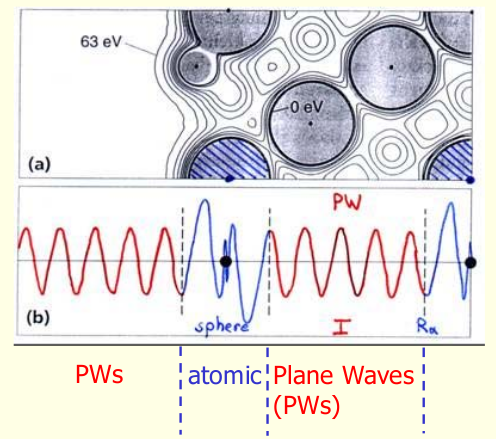
\includegraphics[height=1.30in,width=1.45in,viewport=1 20 485 435,clip]{APW.png}
\caption{\small \textrm{Partitioning of the unit cell into atomic spheres and an interstitial region.}}%(与文献\cite{EPJB33-47_2003}图1对比)
\label{Muffin_tin_0}
\end{figure}
根据MT近似,在WS原胞的每个MT球内,势能具有球对称性$V(r)$,MT球内的基函数表示为:
\begin{equation}
  \varphi(\vec k_i,\vec r)=\sum_{l=0}^{\infty}\sum_{m=-l}^lA_{lm}(\vec k_i)u_l(|\vec r-\vec r_s|)Y_{lm}(\widehat{\vec r-\vec r_s})
  \label{eq:solid-109}
\end{equation}
这里$Y_{lm}$是球谐函数;$\vec k_i=\vec k+\vec G_i$;$\vec G_i$是倒格矢;$\vec r_s$是第$s$个MT球心位置,$A_{lm}$是待定系数;$u_l(\vec r)$是径向Schr\"odinger方程
\begin{equation}
  -\frac1{r^2}\frac d{dr}\left(r^2\frac{du_l}{dr}\right)+\left[\frac{l(l+1)}{r^2}+V(r)\right]u_l=E_l^{\prime}u_l
  \label{eq:solid-110}
\end{equation}
为确定$u_l(r)$,要求$u_l(r)$的边条件$r$=0是非奇异的,但在MT球面$r$=$R_{MT}^s$上,没有对$u_l(r)$加任何限制条件,因此能量式\eqref{eq:solid-110}中的$E_l^{\prime}$可以取任意值。

在MT球外的间隙区,MT势能取为0,间隙区的基函数为:
\begin{equation}
	\varphi(\vec k_i,\vec r)=\exp\mathrm{i}\vec k_i\vec r=\exp\mathrm{i}\vec k_i\cdot(\vec r_s+\vec r)
  \label{eq:solid-111}
\end{equation}
将平面波用球谐函数展开,
\begin{equation}
	\exp\mathrm{i}\vec k_i\cdot\vec r=4\pi\sum_{l=0}^{\infty}\sum_{m=-l}^l\mathrm{i}^lj_l(|\vec k_i|r)Y_{lm}^{\ast}(\hat{\vec k}_i)Y_{lm}(\hat{\vec r})
  \label{eq:solid-112}
\end{equation}
这里$j_l(|\vec k_i|r)$是第$l$阶球Bessel函数;$\hat{\vec k}_i$和$\hat{\vec r}$是矢量$\vec k$和$\vec r$与$z$轴的夹角对应球坐标角度部分$\theta$和$\phi$。

为了使得基函数在球面上连续条件,要求式\eqref{eq:solid-109}和\eqref{eq:solid-111}在球面上数值相等,由此可确定系数$A_{lm}(\vec k_i)$:
$$A_{lm}(\vec k_i)=4\pi e^{\mathrm{i}\vec k_i\cdot\vec r_s}\mathrm{i}^lY_{lm}(\hat{\vec k}_i)j_l(|\vec k_i|R_{MS}^s)/u_l(E,R_{MT}^s)$$
所以APW的基组可以表示为:
\begin{equation}
  \begin{split}
    \varphi&(\vec k_i,\vec r)\\
    &=\left\{\begin{aligned}
	    &e^{\mathrm{i}\vec k_i\cdot\vec r_s}e^{\mathrm{i}\vec k_i\cdot\vec r},&|\vec r|>R_{MT}^s\\
    &4\pi e^{\mathrm{i}\vec k_i\cdot\vec r_s}\sum_{lm}\mathrm{i}^lj_l(|\vec k_i|R_{MS}^s)Y_{lm}^{\ast}(\hat{\vec k}_i)Y_{lm}(\hat{\vec r})u_l(r,E^{\prime})/u_l(R_{MT}^s,E^{\prime}),\quad&|\vec r|\leqslant R_{MT}^s
    \end{aligned} \right.
  \end{split}
  \label{eq:solid-113}
\end{equation}

对于基函数在MT球面不连续的情形,用Schlosser和Marcus的能量变分表达式\cite{PR131-2529_1963},
\begin{equation}
  \begin{split}
    E\int_{\mathrm{I+II}}\Psi^{\ast}\Psi dV=&\int_{\mathrm{I+II}}\Psi^{\ast}\mathbf H\Psi dV+\frac12\int_S\left[(\Psi_{\mathrm{II}}-\Psi_{\mathrm I})\frac{\partial}{\partial\rho}\Psi_{\mathrm {II}}^{\ast}+\frac{\partial}{\partial\rho}\Psi_{\mathrm I}^{\ast}\right.\\
    &-(\Psi_{\mathrm {II}}^{\ast}+\Psi_{\mathrm I}^{\ast})\left.\left(\frac{\partial}{\partial\rho}\Psi_{\mathrm{II}}-\frac{\partial}{\partial\rho}\Psi_{\mathrm I}\right)\right]dS
  \end{split}
  \label{eq:solid-114}
\end{equation}
这里I和II分别表示MT球的内(I)外(II)两部分。上式中的前两个积分项表示对整个WS原胞的积分,第三个积分项是对MT球的球面S的积分。$\partial/\partial\rho$沿球面正方向对区域I的偏导。采用连续基函数,则\eqref{eq:solid-114}可以简化为:
\begin{equation}
  \begin{split}
    E\int_{\mathrm{I+II}}\Psi^{\ast}\Psi dV=&\int_{\mathrm{I+II}}\Psi^{\ast}\mathbf H\Psi dV\\
    &-\frac12\int_S(\Psi_{\mathrm {II}}^{\ast}+\Psi_{\mathrm I}^{\ast})\left(\frac{\partial}{\partial\rho}\Psi_{\mathrm{II}}-\frac{\partial}{\partial\rho}\Psi_{\mathrm I}\right)dS
  \end{split}
  \label{eq:solid-115}
\end{equation}
这里的球面积分是考虑波函数$\Psi$在MT球面上导数不连续。

因为APW基函数径向部分与能量参数$E_l$有关,因此矩阵元与$E_l$有关。为了获得能量本征值$E_l$,必须求解$\vec k$-空间中每个点的能量$E_l$高阶行列式,该过程非常麻烦。为了克服基函数对能量$E_l$的相关,人们提出了多种线性化思想\cite{PRB2-3098_1970,PRB2-290_1970,JPF9-661_1979,PRB19-6094_1979}。线性化缀加平面波(linearized augmented plane-wave, LAPW)方法的思想是在某个给定值$E_{l0}$附近对能量作Taylor展开到一阶\cite{PRB12-3060_1975}。由于波函数的线性化引入的误差,比因为对势能近似引入的误差小得多。换句话说,通过引入线性化,可使得固体中价电子径向波函数与能量参数无关。由此得到Hamiltonian和重叠矩阵与能量参数无关。Koelling和Arbman将LAPW方法应用于Cu的计算\cite{JPF5-2041_1975}。Smr\v cka提出了二次APW方法\cite{Smrcka}。
与APW方法相似,LAPW方法的基函数取为:
\begin{equation}
  \varphi(\vec k_j,\vec r)=\left\{
  \begin{aligned}
	  &\Omega_0^{-1/2}\exp{\mathrm{i}\vec k_j\cdot\vec r},&r>R_{MT}^s\\
    &\sum_{lm}[A_{lm}u_l(E_l,r)+B_{lm}\dot u_l(E_l,r)]Y_{lm}(\hat{\vec r}),\quad&r\leqslant R_{MT}^s
  \end{aligned}\right.
  \label{eq:LAPW-basis}
\end{equation}
这里$R_{MT}^s$是MT球半径;$\vec k_j=\vec k+\vec G_j$,$\vec k$是不可约Brillouin区中的波矢;$\vec G_j$是倒空间格矢;$u_l(E_l,r)$是满足能量为$E_l$的径向Schr\"odinger方程的解波函数;$\dot u_l(E_l,r)$是解波函数对能量$E_l$的一阶导数;$Y_{lm}$是球谐函数;$\Omega_0$是WS原胞体积。与APW不同,这里$E_l$是指定范围内的能量参数,而非变量。不同的角动量$l$可指定不同的能量。关于APW/LAPW方法基函数(径向部分)在球面上的衔接如图\ref{Muffin_tin}所示。
\begin{figure}[h!]
\centering
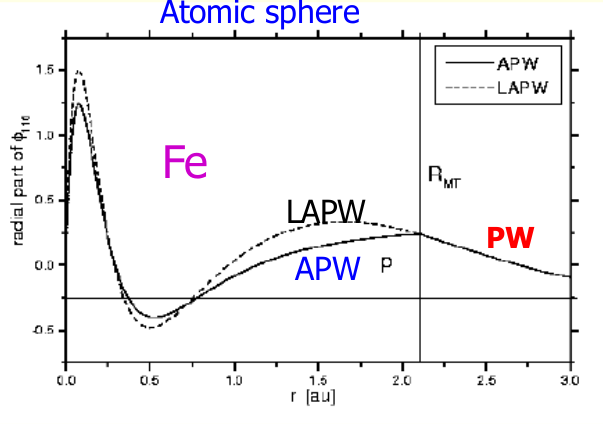
\includegraphics[height=1.30in,width=1.98in,viewport=1 20 585 435,clip]{WIEN2k-LAPW.png}
\caption{\small \textrm{Partitioning of the unit cell into atomic spheres(I) and an interstitial region(II)}}%(与文献\cite{EPJB33-47_2003}图1对比)
\label{Muffin_tin}
\end{figure}

为了提高LAPW方法的线性化程度(即提高基组的变分自由度),在同一能量范围处理半芯态(接近价态的能量较高的芯态)和价态,可采用外加基函数(与$\vec k$无关)方案,这部分外加基函数称为局域轨道(local orbitals, LO)\cite{PRB43-6388_1991,Singh}。由此构造的基函数包含两个指定能量的径向波函数和其中一个能量导数,这样的基函数即LAPW-LO:
\begin{equation}
  \phi_{lm}^{LO}(\vec r)=[A_{lm}u_l(E_{1,l},r)+B_{lm}\dot u_l(E_{1,l},r)+C_{lm}u_l(E_{2,l},r)]Y_{lm}(\hat{\vec r})
  \label{eq:LAPW-LO}
\end{equation}
根据条件$\phi_{lm}^{LO}$在MT球面上数值为零且保持一阶导数连续,并要求$\phi_{lm}^{LO}$在MT球内归一化,可以确定系数$A_{lm}$,$B_{lm}$,$C_{lm}$。

Sj\"ostedt等\cite{SSC114-15_2000}的计算表明,在标准LAPW方法中,将平面波展开使之在MT球面上与球内函数数值和一阶导数连续,这并非是实现Slater型APW方法最有效的线性化方法。采用指定能量参数$E_l$的APW形式的径向波函数[式\eqref{eq:APW-basis}],外加APW型局域轨道(local orbit, lo)扩展基函数,是更有效的方案,称为APW+lo。
\begin{equation}
  \varphi_{\vec k_i,\vec r}=\sum_{lm}[A_{lm}(\vec k_i)u_l(E_l,r)]Y_{lm}(\hat{\vec r})
  \label{eq:APW-basis}
\end{equation}
\begin{equation}
  \phi_{lm}^{lo}=[A_{lm}u_l(E_{1,l})+B_{lm}\dot u_l(E_{1,l})]Y_{lm}(\hat{\vec r})
  \label{eq:APW-lo}
\end{equation}
APW+lo基函数式\eqref{eq:APW-lo}形式上与标准LAPW式\eqref{eq:LAPW-basis}形式非常相似,但这里系数$A_{lm}$和$B_{lm}$与$\vec k$无关,是根据式\eqref{eq:APW-lo}在MT球边界上数值为零并且在MT球内归一化确定。这样构造的APW+lo基函数,总的波函数在MT球面上平滑且一阶可导的,但是根据式\eqref{eq:solid-115},在MT球面上有动能部分对Hamiltonian的贡献。为收敛到相同的结果,采用APW+lo基组比起标准LAPW基组小得多\cite{PRB64-195134_2001}。因此选择APW+lo基组比标准LAPW基组的计算效率要高。

%WIEN2K程序包建议\cite{CPC59-399_1990,WIEN2K-UG_2001,CPC147-71_2002}一般平面波基函数收敛缓慢的轨道(比如过渡金属的3d态波函数)或MT球半径特别小的体系用APW+lo基组展开,其余价电子轨道用LAPW基组展开,此外对必要的半芯层可以用LO基组展开。用这样的方式可以同时考虑价态和半芯态。

\subsection{FP-LAPW的总能计算}
根据\textrm{APW}方法的基本思想,原子的芯电子的运动限于\textrm{MT}球内,价电子的运动范围遍及\textrm{MT}球区和间隙区。材料的物理和化学性质主要取决于体系的价电子状态,\textrm{WIEN2k}程序处理价电子时,对应的基函数在空间的不同位置采用不同的表示。

所谓全势(\textrm{Full-potential})方法的思想,简言之,就是无论价电子在\textrm{MT}球区,还是在间隙区,感受到的都是包括芯层电子在内的其他电子的排斥势和各格点原子核的吸引势。原则上,对于周期性体系,已知体系的电荷密度分布,由\textrm{Poisson}方程,可以直接求得体系的\textrm{Coulomb}势。众所周知,由于靠近原子核的区域,电荷密度(及相应的\textrm{Coulomb}势)变化剧烈,因此直接的\textrm{Fourier}级数展开不易收敛。为了克服这一困难,\textrm{Weinert}\cite{JMP22-2433_1981}注意到间隙区的电子\textrm{Coulomb}相互作用只和间隙区的电荷密度及\textrm{MT}球区的电荷多极矩(\textrm{multipole moments})有关。它的基本思想是利用电荷多极矩和球形边界\textrm{Dirichlet}边值问题求解\textrm{MT}球内的\textrm{Coulomb}势分布,进而得到间隙区\textrm{Coulomb}势的分布。

注意到\textrm{MT}球内电荷对间隙区势能的贡献\cite{Jackson}:
\begin{equation}
	V(r)=\sum_{l=0}^{\infty}\sum_{m=-l}^{l}\dfrac{4\pi}{2l+1}q_{lm}\dfrac{Y_{lm}(\hat r)}{r^{l+1}}
	\label{eq_V-multi-mom}
\end{equation}
这里,$q_{lm}$是\textrm{MT}球内的电荷多极矩。
%\begin{equation}
%	\rho_I(\vec r)=\sum_{\vec K}\rho_I(\vec K)\mathrm{e}^{\mathrm{i}\vec K\cdot\vec r}
%	\label{eq_rho_i_four}
%\end{equation}

在实际计算中,\textrm{MT}区球内的电荷多极矩$q_{lm}$由下式给出:
\begin{equation}
	q_{lm}=\int_{S}Y_{lm}^{\ast}(\hat r)r^l\rho(r)\mathrm{d}^3r
	\label{eq_multi-mom}
\end{equation}
因此有可能重构\textrm{MT}球区的电荷密度分布,使它既有与实际电荷密度分布相同的电荷多极矩,又能有较好的\textrm{Fourier}收敛行为。
\begin{equation}
	\rho(\vec r)\rightarrow\tilde\rho(\vec r)=\rho_I(\vec r)\theta(\vec r\in I)+\sum_{spheres}\tilde\rho_i(\vec r)\theta(\vec r\in S_i)
	\label{eq_pseudo-rho}
\end{equation}
间隙区电荷密度$\rho_I(\vec r)$变化平缓,可用方便地作\textrm{Fourier}级数展开:
\begin{equation}
	\rho_I(\vec r)=\sum_{\vec K}\rho_I(\vec K)\mathrm{e}^{\mathrm{i}\vec K\cdot\vec r}
	\label{eq_rho_i_four}
\end{equation}

如果将间隙区的电荷密度延伸到\textrm{MT}球内,于是体系的电荷密度表示为:
\begin{equation}
	\rho(\vec r)=\rho_I(\vec r)+\sum_{spheres}\big[\rho_i(\vec r)-\rho_I(\vec r)\big]\theta(\vec r\in S_i) 
	\label{eq_rho_rean}
\end{equation}
此时$\rho_I(\vec r)$可在整个空间作\textrm{Fourier}展开。其中延伸到\textrm{MT}球内(球心位置记作$\xi_i$)的间隙区电荷密度表示为:
\begin{equation}
	\rho_I(\vec r)=\sum_{\vec K}\rho_I(\vec K)\mathrm{e}^{\mathrm{i}\vec K\cdot\vec\xi_i}\mathrm{e}^{\mathrm{i}\vec K\cdot\vec r_i} 
	\label{eq_rho_i_four_i}
\end{equation}
这里$\vec r_i=\vec r-\xi_i$。

如果已知\textrm{MT}球内的真实电荷密度分布,第$i$个\textrm{MT}球内多极矩记作$q_{lm}^i$。
%\begin{equation}
%	q_{lm}^{Ii}=\biggl\{
%	\begin{aligned}
%		&\dfrac{\sqrt{4\pi}}3R_i^3\rho_I(K=0)\delta_{l0}\quadd \\
%		&4\pi\mathrm{i}^l\sum_{\vec K\neq 0}\rho_I(\vec K)\dfrac{R_i^{l+3}j_{l+1}(\vec K\cdot\vec R)}{KR_i}\mathrm{e}^{\mathrm{i}\vec K\cdot\xi_i}Y_{lm}^{\ast}(\hat K)
%	\end{aligned}\biggr.
%	\label{eq_multi_PW}
%\end{equation}
延伸到球内的间隙区电荷对球内多极矩的贡献即为:
\begin{equation}
	q_{lm}^{Ii}=\dfrac{\sqrt{4\pi}}3R_i^3\rho_I(K=0)\delta_{l0}+4\pi\mathrm{i}^l\sum_{\vec K\neq 0}\rho_I(\vec K)\dfrac{R_i^{l+3}j_{l+1}(\vec K\cdot\vec R)}{KR_i}\mathrm{e}^{\mathrm{i}\vec K\cdot\xi_i}Y_{lm}^{\ast}(\hat K)
	\label{eq_multi_PW}
\end{equation}
这里利用了平面波在球心$\xi_i$处的球谐函数展开关系:
\begin{equation}
	\mathrm{e}^{\mathrm{i}\vec K\cdot \vec r}=\sum_{lm}4\pi\mathrm{i}^lj_l(\vec K\cdot\vec r)Y_{lm}^{\ast}(\hat{\vec K})Y_{lm}(\hat{\vec r})
	\label{eq_PW_Bessel}
\end{equation}
和积分表达式:
\begin{equation}
	\int_0^R r^{l+2}j_l(\vec K\cdot\vec r)\mathrm{d}r=\left\{
	\begin{aligned}
		&\dfrac{R^3}3\delta_{l,0}\quad &\vec K=0\\ 
		&\dfrac{R^{l+3}j_{l+1}(\vec K\cdot\vec R)}{KR} &\vec K\neq 0
	\end{aligned}\right.
	\label{eq_int_r_j}
\end{equation}

因此,重构方程\eqref{eq_rho_rean}在\textrm{MT}球内的电荷密度分布,其多极矩满足:
\begin{equation}
	\tilde q_{lm}^i=q_{lm}^i-q_{lm}^{Ii}
	\label{eq_psmult}
\end{equation}
根据文献\onlinecite{JMP22-2433_1981},可以得到重构的\textrm{MT}球内的赝电荷密度的\textrm{Fourier}展开系数为:
\begin{equation}
	\tilde\rho_s(\vec K)=\dfrac{4\pi}{\Omega}\sum_{lm,i}\dfrac{(-\mathrm{i})^l(2l+2n+3)!!}{(2l+1)!!}\times\dfrac{j_{l+n+1}(\vec K\cdot\vec R_i)}{(KR_i)^{n+1}}\tilde q_{lm}^i\mathrm{e}^{-\mathrm{i}\vec K\cdot\vec\xi_i}Y_{lm}(\hat K)
	\label{eq_psrho}
\end{equation}
这里$n$是整数。$\tilde\rho_s(\vec K)$可以视为$n$的函数,文献\onlinecite{JMP22-2433_1981}讨论了对于不同的$l$和$(\vec K\cdot\vec R_i)_{max}$,优化$n$值得到最佳收敛的$\tilde\rho_s(\vec K)$的情况。一般取$n=\big[\dfrac12(\vec K\cdot\vec R_i)_{max}\big]$,\textrm{WIEN2k}程序中取$n=9$。

当$\vec K=0$,有
$$\tilde\rho_s(\vec K=0)=\dfrac{\sqrt{4\pi}}{\Omega}\sum\limits_i\tilde q_{00}^i$$
因此,用于计算间隙区\textrm{Coulomb}势的赝电荷密度(较平缓)可写成\textrm{Fourier}展开形式:
\begin{equation}
	\tilde\rho(\vec r)=\sum_{\vec K}\big[\rho_I(\vec K)+\tilde\rho_s(\vec K)\big]\mathrm{e}^{\mathrm{i}\vec K\cdot\vec r}
	\label{eq_psrho_four}
\end{equation}
求解\textrm{Poisson}方程,间隙区的\textrm{Coulomb}势表达式为:
\begin{equation}
	V_I(\vec r)=\sum_{\vec K}\dfrac{4\pi}{K^2}\big[\rho_I(\vec K)+\tilde\rho_s(\vec K)\big]\mathrm{e}^{\mathrm{i}\vec K\cdot\vec r}
	\label{eq_Vcou_I}
\end{equation}
与此同时,根据文献\onlinecite{JMP22-2433_1981},已知球面上的\textrm{Coulomb}势,根据\textrm{Dirichlet}的球形边值问题\cite{Jackson},可知\textrm{MT}球内的\textrm{Coulomb}势的表达式\cite{Singh,Nemoshkalenko-Antonov}为:
\begin{equation}
	\begin{aligned}
		V_s(\vec r)=&\sum_{lm}Y_{lm}(\hat r)\left[\dfrac{4\pi}{2l+1}\left\{\dfrac1{r^{l+1}}\int_0^r\mathrm{d}r^{\prime}(r^{\prime})^{l+2}\rho_{lm}(r^{\prime})+r^l\int_r^{R_i}\mathrm{d}r^{\prime}(r^{\prime})^{1-l}\rho_{lm}(r^{\prime})\right\}\right.\\
		&\left.+\left(\dfrac r{R_i}\right)^l4\pi\mathrm{i}^l\sum_{\vec K\neq0}\dfrac{4\pi}{K^2}\tilde\rho_s(\vec K)Y_{lm}^{\ast}(\vec K)\dfrac{\vec K\cdot\vec R_ij_{l-1}(\vec K\cdot\vec R_i)}{2l+1}\right]
	\end{aligned}
	\label{eq_Vcou_s}
\end{equation}
%球面$R_i$上的\textrm{Coulomb}势可以表达为
%\begin{equation}
%	V_{l=0}(R_i)=4\pi\sum_{\vec K\neq0}\dfrac{\vec K\cdot\vec R_i\tilde\rho_s(\vec K)}{K^2}Y_{00}^{\ast}(\vec K)j_0(\vec K\cdot\vec R_i)
%	\label{eq_Vcou_S}
%\end{equation}

注意到由于\textrm{MT}球的存在,倒空间不连续,即
\begin{equation}
	V_I(\vec r)=\left\{\sum_{\vec K}\dfrac{4\pi}{K^2}\bigg[\tilde\rho_I(\vec K)+\tilde\rho_s(\vec K)\bigg]\mathrm{e}^{\mathrm{i}\vec K\cdot\vec r}\right\}\theta(r)\qquad(r\in \mathrm{Interstitial})
	\label{eq_Vcou_I_theta}
\end{equation}
%由于间隙区的势能变化平缓,基函数是平面波,因此可以\textbf{重新定义能量零点,先将$V_C(\vec K=0)$置为零。}
倒空间中的势能表示为:
\begin{equation}
	V_I(\vec K)=\left\{
	\begin{aligned}
		&\mathrm{divergence} \qquad &\vec K=0 \\
		\dfrac{(4\pi)^2}{K^3}\bigg[\rho_I(\vec K)+&\tilde\rho_s(\vec K)\bigg]\sum_i\dfrac{R_i^2j_1(\vec K\cdot\vec R_i)}{\Omega}\mathrm{e}^{-\mathrm{i}\vec K\cdot\vec\xi_i}\quad &\vec K\neq0
	\end{aligned}\right.
	\label{eq_Vcou_KI_theta}
\end{equation}
显然,由于$\vec K=0$项的存在,使得间隙区的电子\textrm{Coulomb}势具有发散性。
%在\textrm{MT}球内,按照原子\textrm{Coulomb}相互作用表达式可以参考文献\onlinecite{Singh,Nemoshkalenko-Antonov}。

综上所述,\textrm{LAPW}方法中在\textrm{MT}球内和间隙区分别采用\eqref{eq_Vcou_s}和\eqref{eq_Vcou_I_theta}的势函数形式,实现全势(\textrm{full potential})\cite{PRB26-4571_1982,PRB33-823_1986}计算。
%一般是在每个\textrm{MT}球内,势函数用球谐函数(或者是满足晶体对称性的球谐函数)展开,MT球外的势函数用\textrm{Fourier}级数展开\cite{PRB13-5362_1976}

引入\textrm{Madelung}势,完成总能量的计算过程\cite{JMP22-2433_1981}:
\begin{equation}
	\begin{aligned}
	E_T[\rho]=&T_s[\rho]+U[\rho]+E_{xc}[\rho]\\
	=&T_s[\rho]+\dfrac12\biggl[\int\dfrac{\rho(\vec r)\rho(\vec r^{\prime}){}}{|\vec r-\vec r^{\prime}|}\mathrm{d}\vec r\mathrm{d}\vec r^{\prime}-2\sum_{\alpha}Z_{\alpha}\int\dfrac{\rho(\vec r)\mathrm{d}\vec r}{|\vec r-\vec R_{\alpha}|}+\sideset{}{^\prime}\sum_{\alpha,\beta}\dfrac{Z_{\alpha}Z_{\beta}}{|\vec R_{\alpha}-\vec R_{\beta}|}\biggr]\\
	&+E_{xc}[\rho]\\
	=&T_s[\rho]+\dfrac{N}2\bigg[\int_{\Omega}\rho(\vec r)V_c(\vec r)\mathrm{d}\vec r-\sum_{\nu}Z_{\nu}V_M(\vec\gamma_{\nu})\biggr]+E_{xc}[\rho]
	\end{aligned}
	\label{eq_E_total}
\end{equation}
这里$V_c(\vec r)$是\textrm{Coulomb}势:
\begin{equation}
	V_c(\vec r)=\int\dfrac{\rho(\vec r^{\prime})}{|\vec r-\vec r^{\prime}|}\mathrm{d}\vec r^{\prime}-\sum_{\alpha}\dfrac{Z_{\alpha}}{|\vec r-\vec R_{\alpha}|}
	\label{eq_Vcou_WIEN}
\end{equation}
$V_M(\vec\gamma_{\nu})$是\textrm{Madelung}势:
\begin{equation}
	V_M(\vec\gamma_{\nu})=\int\dfrac{\rho(\vec r)\mathrm{d}\vec r}{|\vec r-\vec\gamma_{\nu}|}-\sideset{}{^\prime}\sum_{\alpha}\dfrac{Z_{\alpha}}{|\vec R_{\alpha}-\vec\gamma_{\nu}|}
	\label{eq_Vmadelung}
\end{equation}
即将离子相互作用、电子间相互作用和离子-电子相互作用分为电子感受的\textrm{Coulomb}势和原子核位置的\textrm{Madelung}势贡献。因此利用电子的\textrm{Coulomb}势与\textrm{Madelung}势在球心处的贡献的球形部分彼此抵消来排除奇点:

球心位于$\vec\gamma_{\nu}$、半径为$R_{\nu}$的\textrm{MT}球球面上的势能平均值$S_0(R)$可由式\eqref{eq_Vcou_s}计算,因此除去球心核电荷以外所有电荷在MT球面上产生的势能平均为:
\begin{equation}
  S(R_{\nu})\equiv S_0(R_{\nu})+Z_{\nu}/R_{\nu}
  \label{eq:solid-79}
\end{equation}
因此球心$\vec\gamma_{\nu}$处的\textrm{Madelung}势的球对称部分贡献为\cite{PRB26-4571_1982}:
\begin{equation}
  \begin{split}
	  V_M(\vec\gamma_{\nu})&=\frac1{R_{\nu}}\big[R_{\nu}S_0(R_{\nu})+Z_{\nu}-Q_{\nu}\big]+\sqrt{4\pi}\int_0^{R_{\nu}}\mathrm{d}rr\rho_{00}(r)\\
	   &=\frac1{R_{\nu}}\big[R_{\nu}S_0(R_{\nu})+Z_{\nu}-Q_{\nu}\big]+\bigg\langle\frac1r\rho(\vec r)\bigg\rangle_{\nu}
  \end{split}
   \label{eq:Madelung}
\end{equation}
其中$Q_{\nu}$表示\textrm{MT}球内的电子电荷之和。$\rho(\vec r)$是\textrm{MT}球内的电荷密度,可以用球谐函数表示为:
\begin{equation}
  \rho(\vec r_{\nu})=\sum_{lm}\rho_{lm}(r_{\nu})Y_{lm}(\hat r_{\nu})
  \label{eq:solid-80}
\end{equation}
因此\textrm{MT}球内的总能量贡献为:
\begin{equation}
  \begin{split}
	  E_T=\sum_i\varepsilon_i&-\frac12\int_{\Omega}\rho(\vec r)\big[V_c(\vec r)+\mu_{xc}(\vec r)\big]\mathrm{d}\vec r-\frac12\sum_{\nu}Z_{\nu}V_M(\vec\gamma_{\nu})+E_{xc}[\rho] \\
   =\sum_i\varepsilon_i&-\frac12\left(\int_{\Omega}\rho(\vec r)V_c(\vec r)\mathrm{d}\vec r+\sum_{\nu}Z_{\nu}\bigg\langle\frac1r\rho(\vec r)\bigg\rangle_{\nu}\right)-\dfrac12\int_{\Omega}\rho(\vec r)\mu_{xc}(\vec r)\mathrm{d}\vec r\\
   &-\frac12\sum_{\nu}\frac{Z_{\nu}}{R_{\nu}}\big[R_{\nu}S_0(R_{\nu})+Z_{\nu}-Q_{\nu}\big]+E_{xc}[\rho]
  \end{split}
  \label{eq:solid-81}
\end{equation}
这里$V_c(\vec r)=\displaystyle\int\dfrac{\rho(\vec r\,^\prime)}{|\vec r-\vec r\,^\prime|}\mathrm{d}\vec r\,^\prime-\sum\limits_{\alpha}\dfrac{Z_{\alpha}}{|\vec r-\vec R_{\alpha}|}$。总能量写成这样的形式,原子核位置的\textrm{Coulomb}势奇点可以排除。将势能和电荷密度在各原子核附近作球谐展开,在原子核附近,有
\begin{equation}
  \begin{split}
	  &\int_{\Omega}\rho(\vec r)V_c(\vec r)\mathrm{d}\vec r+Z_{\nu}\sqrt{4\pi}\int_0^{R_{\nu}}\mathrm{d}rr^2\frac{\rho_{00}(r)}r\\
	  =&\sqrt{4\pi}\int\mathrm{d}rr^2\rho_{00}(r)\left[V_{00}(r)Y_{00}(\hat r)+\frac{Z_{\nu}}r\right]+\sum_{lm>0}\int\mathrm{d}rr^2\rho_{lm}(r)V_{lm}(r)
  \end{split}
\end{equation}
\textrm{Coulomb}势的奇点只出现在$V_{00}(r)$中,将$V_{00}(r)$写成核的点电荷势与源于电子的平滑势两部分之和,有
$$V_{00}(r)=-\sqrt{4\pi}\frac{Z_{\nu}}r+\hat V_{00}(r)$$
通过这样的方式,可以将总能量中的奇点排除,但同样单独\textrm{Coulomb}势和\textrm{Madelung}势每一项在原子核位置能量仍然是发散的。

%如果采用标准的\textrm{LDA}近似,式\eqref{eq:solid-81}交换-相关能可以写成:
%\begin{equation}
%  E_{xc}[\rho]\approx\int_{\Omega}\rho(\vec r)\varepsilon_{xc}(\vec r)d\vec r
%  \label{eq:solid-82}
%\end{equation}
基于\textrm{LAPW}方法的总能量计算,在空间中不同的区域采用不同的表示。%间隙区(\textrm{I})的电荷密度用平面波展开,有
%$$\rho(\vec r)=\sum_{\vec G}\rho(\vec G)e^{i\vec G\cdot\vec r},\quad \vec r\in\mathrm{I}$$
%在\textrm{MT}球内,电荷密度用球谐函数展开,在动量空间中的展开形式为:
%$$\bar\rho_{lm}(r_{\nu})=4\pi i^l\sum_{\vec G}\rho(\vec G)e^{i\vec G\cdot\vec r_{\nu}}j_l(Gr_{\nu})Y_{lm}^{\ast}(\vec G)$$ 
首先,将间隙区$V_C(\vec K=0)$置零,排除间隙区的\textrm{Coulomb}势$V_I(\vec K)$的奇点:
\begin{equation}
	\tilde V_I(\vec K)=\left\{
	\begin{aligned}
		&0 \qquad &\vec K=0 \\
		\dfrac{(4\pi)^2}{K^3}\big[\rho_I(\vec K)+&\tilde\rho_s(\vec K)\big]\sum_i\dfrac{R_i^2j_1(\vec K\cdot\vec R_i)}{\Omega}\mathrm{e}^{\mathrm{i}\vec K\cdot(\vec r-\vec\xi_i)}\quad &\vec K\neq0
	\end{aligned}\right.
	\label{eq_Vcou_KI_theta_2}
\end{equation}
%在总能量计算中补偿这一平移。
\textrm{MT}球内对总能量的贡献部分在正空间中按上述式\eqref{eq:solid-81}计算。

因此\textrm{LAPW}方法的原胞内的晶体总能量可以写成:
\begin{equation}
  \begin{split}
	  E=&\sum_i\varepsilon_i-\sum_{\vec K}\Omega\rho_I(\vec K)\tilde V_I^{\ast}(\vec K)-\frac12\sum_{\nu}\dfrac{Z_{\nu}}{R_{\nu}}[Z_{\nu}-Q_{\nu}+R_{\nu}S_0(R_{\nu})]\\
    &-\sum_{\nu}\sum_{lm}\int_0^{R_{\nu}}\mathrm{d}rr^2\left[\rho_{lm}(r_{\nu})\left(\tilde V_{lm}^{\ast}(r_{\nu})+\dfrac{\sqrt{4\pi}}{2r_{\nu}}Z_{\nu}\delta_{l0}\right)-\bar\rho_{lm}(\vec r_{\nu})\bar V_{lm}^{\ast}(\vec r_{\nu})\right]
  \end{split}
  \label{eq:solid-83}
\end{equation}
这里$\tilde V(\vec r)$和$\bar V_{lm}(\vec r)$根据都按下式计算:
$$\tilde V(\vec r)=\frac12V_c(\vec r)-\varepsilon_{xc}(\vec r)+\mu_{xc}(\vec r)$$

%\textrm{WIEN2k}程序中,\textbf{程序\textrm{lapw0}部分完成式\eqref{eq:solid-83}中除$\sum\limits_i\varepsilon_i$之外的所有各项的计算}。
%\subsection{LDA+U和GW近似}
%\subsubsection{GW近似}
%Landau的Fermi液体理论是研究群体激发和多体Fermi子体系物理性质的重要方法\cite{Landau}。Fermi液体的特征是准粒子分布$\varepsilon=\varepsilon(\vec k)$由体系总能量$E$对分布函数的变分,即
%\begin{equation}
%  \frac{\delta E}{\delta n(\vec k)}=\varepsilon(\vec k)
%  \label{eq:solid-219}
%\end{equation}
%关联函数$f(\vec k,\vec k^\prime)$由准粒子能量对整个$\vec k$空间粒子分布变分得到
%\begin{equation}
%  \frac{\delta\varepsilon(\vec k)}{\delta n(\vec k^\prime)}=\frac{\delta^2E}{\delta n(\vec k)\delta n(\vec k^\prime)}=f(\vec k,\vec k^\prime)
%  \label{eq:solid-220}
%\end{equation}
%考虑准粒子间相互作用,体系激发能记作
%\begin{equation}
%  W=\sum_{\vec k}\varepsilon(\vec k)\delta n(\vec k)+\frac12\sum_{\vec k}\sum_{\vec k^\prime}f(\vec k,\vec k^\prime)\delta n(\vec k)\delta(\veck^\prime)
%  \label{eq:solid-221}
%\end{equation}
%
%Green函数是研究Fermi液体的重要数学工具。对宏观体系,Green函数定义为\cite{Lifshitz}
%\begin{equation}
%  \tilde G(x,x^\prime)=-i\langle T\hat\Psi(x)\hat\Psi^{\ast}(x^\prime)\rangle
%  \label{eq:solid-222}
%\end{equation}
%这里$x$表示时间$t$和位置$\vec r$,$\langle\cdots\rangle$表示对体系基态求平均,$T$表示按时间先后乘积算符。$\hat\Psi$是Heisenberg算符,对式\eqref{eq:solid-222}进行Fourier变换,得到以$\vec r$,$E$为表象的Green函数$\tilde G(\vec r,\vec r\,^\prime;E)$是Dyson方程\cite{Lifshitz}
%\begin{equation}
%  (\nabla^2+E)\tilde G(\vec r,\vec r\,^\prime;E)-\int d\vec r^{\prime\prime}\Sigma(\vec r,\vec r^{\prime\prime};E)\tilde G(\vec r^{\prime\prime},\vec r\,^\prime;E)=\delta(\vec r-\vec r\,^\prime)
%  \label{eq:solid-223}
%\end{equation}
%的解。这里$\Sigma(\vec r,\vec r\,^\prime;E)$是描述交换和相关效应的质量或自能算符,这是个与能量有关的非定域的非-Hermitian算符,考虑到粒子与体系中其他粒子的相互作用。晶体中的质量具有平移对称性,
%\begin{equation}
%  \Sigma(\vec r+\vec a,\vec r+\vec a;E)=\Sigma(\vec r,\vec r\,^\prime;E),
%  \label{eq:solid:224}
%\end{equation}
%这里$\vec a$是晶体平移格矢。
%
%临近Green函数的极点,式\eqref{eq:solid-223}右面的$\delta$函数为0,所得积分-微分方程的本征值确定体系激发能谱\cite{Lifshitz,PR145-561_1966}
%\begin{equation}
%  -\delta^2\Phi_{\vec k}(\vec r,E)+\int d\vec r\,^\prime\Sigma(\vec r,\vec r\,^\prime;E)\Phi_{\vec k}(\vec r\,^\prime,E)=\varepsilon_{\vec k}\Phi_{\vec k}(\vec r,E) 
%  \label{eq:solid-225}
%\end{equation}
%这里函数$\Phi_{\vec k}(\vec r,E)$类似于周期场中的单电子Bloch波函数。对金属中的Fermi电子液体中用式\eqref{eq:solid-225}替代一般Schr\"odinger方程。与一般的Schr\"odinger方程不同,式\eqref{eq:solid-225}的能量本征值是复数,因为质量算符$\Sigma(\vec r,\vec r\,^\prime;E)$是复数。
%
%由式(\ref{eq:solid-223},\ref{eq:solid-225})得到Green函数
%\begin{equation}
%  \tilde G(\vec r,\vec r\,^\prime;E)=\sum_{\vec k}\frac{\Phi_{\vec k}(\vec r,E)\Phi_{\vec k}^{\ast}(\vec r\,^\prime,E)}{E-\varepsilon_{\vec k}(E)+i0\mathrm{sign}E}
%  \label{eq:solid-226}
%\end{equation}
%$\varepsilon_{\vec k}(E)$是体系中加入一个粒子引起的能量改变。如果将单个准粒子改变引起得能量变化$\varepsilon_{\vec k}(E)$定义为式\eqref{eq:solid-219}中的准粒子能量,对临近Fermi面的态,函数$\tilde G(\vec r,\vec r\,^\prime;E)$在$E=\varepsilon_{\vec k}(E)$有极值。因此Green函数极值确定了多Fermi子体系的元激发能谱。一般说,因为和其他粒子相互作用,准粒子能量为复数。复数能量使得体系激发态的寿命有限$(\tau\sim1/|\mathrm{Im}\varepsilon|)$\cite{Landau-Lifshitz}。能量宽度由$\mathrm{Im}\varepsilon$确定。
%
%%临近Fermi能级,$\mathrm{Im}\varepsilon_{\vec k}(E)\rightarrow0$,相应的$\mathrm{Im}\Sigma\rightarrow0$,于是解方程\eqref{eq:solid-225}得到$\mathrm{Re}\varepsilon_{\vec k}(E)$和实数形式的$\Sigma(\vec r,\vec r\,^\prime;E)$和$\epsilon_{\vec k}(E)$。
%
%根据Hohenberg-Kohn定理,本征值$\Sigma(\vec r,\vec r\,^\prime;E)$由体系基态确定,它也是电子密度的函数。Sham和Kohn建议可用局域电子密度近似表示$\Sigma(\vec r,\vec r\,^\prime;E)$\cite{PR145-561_1966}:
%\begin{equation}
%  \Sigma(\vec r,\vec r\,^\prime;E)=V_C(\vec r)\delta(\vec r-\vec r\,^\prime)+\Sigma_0(\vec r-\vec r\,^\prime;E-V_C(\vec r_0);\rho(\vec r_0))
%  \label{eq:solid-227}
%\end{equation}
%这里$\Sigma_0$是密度为$\rho$的无相互作用电子气的本征能量,$V_C(\vec r_0)$是位于$\vec r_0=(\vec r+\vec r\,^\prime)/2$的静电Coulomb势。此外式\eqref{eq:solid-227}已将能量$\Sigma$中的局域部分以Hartree势的形式分离出来,因此可以利用$\Sigma_0$的短程效应。
%
%对本征函数$\Phi_{\vec k}$作近似
%$$\Phi_{\vec k}(\vec r,E)=A(\vec k)\exp[i\vec p(\vec r)\vec r]$$
%并认为$A$和电子动量与$\vec r$无关,将式\eqref{eq:solid-225}称为类似Kohn-Sham方程的表达式\cite{JPC4-2064_1971},
%\begin{equation}
%  [-\nabla^2+V_C(\vec r)+\Sigma_{xc}(\rho(\vec r),E)]\Phi_{\vec k}(\vec r,E)=\varepsilon_{\vec k}(\vec r,E)
%  \label{eq:solid-228}
%\end{equation}
%若$E=\mu$,$\Sigma_{xc}(\rho(\vec r),\mu)\equiv\mu_{xc}(\rho(\vec r))$我们因此得到符合局域密度近似的DFT方程,两者的交换-相关势$\mu_{xc}$是相同的。因此对于低激发能,可以使用近似$\Sigma_{xc}(\rho(\vec r),E)\simeq\mu_{xc}$,此结果对应于忽略准粒子间的相互作用,即Landau函数$f(\vec k,\vec k^\prime)=0$。
%
%因此基于DFT的能带计算,如果充分考虑交换-相关效应,可以计算多电子体系的元激发能量。注意,采用单电子近似,要求能带比较宽,即中心位于不同格点的波函数有较大的重叠,电子间相互作用不是很强。
%
%Hedin和Lundqvist详细回顾了用Green函数技术解决电子相关的问题\cite{Hedin-Lundqvist}。在单粒子近似下的Green函数,准粒子与谱函数的峰联系在一起。如果峰足够尖锐,表明存在一个明确的准粒子能量,对一般的非均匀体系,准粒子能量和波函数可以通过解Dyson方程\eqref{eq:solid-225}求得。对于准粒子问题,核心问题是对自能算符$\Sigma(\vec r,\vec r\,^\prime;E)$的足够好的近似。常用的方法是GW近似\cite{PR139-A796_1965},自能用屏蔽相互作用$W$计算到最低阶。
%\begin{equation}
%  \Sigma(\vec r,\vec r\,^\prime;E)=\frac i{2\pi}\int_{-\infty}^{\infty}dE^\prime\tilde G(\vec r,\vec r\,^\prime;E+E^\prime)W(\vec r,\vec r\,^\prime;E^\prime)
%  \label{eq:solid-229}
%\end{equation}
%Green函数$\tilde G$由准粒子的波函数和能量表示,屏蔽Coulomb作用$W$
%\begin{equation}
%  W(\vec r,\vec r\,^\prime;E)=\frac1{\Omega}\int d^3r^{\prime\prime}\varepsilon^{-1}(\vec r,\vec r^{\prime\prime};E)V(\vec r^{\prime\prime}-\vec r\,^\prime)
%  \label{eq:solid-230}
%\end{equation}
%这里$V$是未屏蔽的Coulomb势,$\varepsilon^{-1}$是介电函数矩阵的逆阵,
%\begin{equation}
%  \varepsilon^{-1}(\vec r,\vec r\,^\prime;E)=\delta(\vec r-\vec r\,^\prime)+\int d^3r^{\prime\prime} V(\vec r\,^\prime-\vec r^{\prime\prime})P(\vec r^{\prime\prime},\vec r\,^\prime;E)
%  \label{eq:solid-231}
%\end{equation}
%这里$P$是完全响应函数,于是
%\begin{equation}
%  W(\vec r,\vec r\,^\prime;E)=V(\vec r-\vec r\,^\prime)+W_c(\vec r,\vec r\,^\prime;E)
%  \label{eq:solid-232}
%\end{equation}
%这里
%\begin{equation}
%  W_c(\vec r,\vec r;E)=\int d^3r_1d^3r_2V(\vec r\,^\prime-\vec r_1)P(\vec r_1,\vec r_2;E)V(\vec r_2-\vec r\,^\prime)
%  \label{eq:solid-233}
%\end{equation}
%Green函数可以写成谱表示
%\begin{equation}
%  G(\vec r,\vec r\,^\prime;E)=\int_{-\infty}^{\mu}dE^\prime\frac{A(\vec r,\vec r\,^\prime;E^\prime)}{E-E^\prime-i\delta}+\int_{\mu}^{\infty}dE^\prime\frac{A(\vec r,\vec r\,^\prime;E^\prime)}{E-E^\prime+i\delta}
%  \label{eq:solid-234}
%\end{equation}
%这里$A(\vec r,\vec r\,^\prime;E)=-\frac1{\pi}\mathrm{Im}G(\vec r,\vec r\,^\prime;E)\mathrm{sgn}(E-\mu)$
%
%实际计算中,取零阶Green函数,有
%\begin{equation}
%  A(\vec r,\vec r\,^\prime;E)=\sum_{kn}\psi_{kn}(\vec r)\psi_{kn}^{\ast}(\vec r\,^\prime)\delta(E-E_{kn})
%  \label{eq:solid-235}
%\end{equation}
%于是自能可以写成
%\begin{equation}
%  \Sigma(\vec r,\vec r\,^\prime;E)=\Sigma_x(\vec r,\vec r\,^\prime)+\Sigma_c(\vec r,\vec r\,^\prime;E)
%  \label{eq:solid-236}
%\end{equation}
%这里$\Sigma_x$是净的交换势,
%\begin{equation}
%  \Sigma_x(\vec r,\vec r\,^\prime)=-\sum_{kn}^{occ}\psi_{kn}(\vec r)\psi_{kn}^{\ast}(\vec r\,^\prime)V(\vec r-\vec r\,^\prime)
%  \label{eq:solid-254}
%\end{equation}
%$E_c$自能的相关部分,
%\begin{equation}
%  \begin{split}
%    \Sigma_c(\vec r,\vec r\,^\prime;E)=&\sum_{kn}^{occ}\psi_{kn}(\vec r)\psi_{kn}^{\ast}(\vec r\,^\prime)W_c^-(\vec r,\vec r\,^\prime;E-E_{kn})\\
%    &+\sum_{kn}^{occ}\psi_{kn}(\vec r)\psi_{\vec r}^{\ast}(\vec r\,^\prime)W_c^+(\vec r,\vec r\,^\prime;E-E_{kn})
%  \end{split}
%  \label{eq:solid-237}
%\end{equation}
%其中$W_c^{\pm}(\vec r,\vec r\,^\prime;E)=\dfrac i{2\pi}\displaystyle\int_{-\infty}^{+\infty}dE^\prime\frac{W_c(\vec r,\vec r\,^\prime;E^\prime)}{E+E^\prime\pm i\delta}$。于是$\Sigma(\vec r,\vec r\,^\prime;E)$可以记作\cite{JPCM9-767_1997},
%\begin{displaymath}
%  \Sigma(\vec r,\vec r\,^\prime;E)=-\sum_{kn}\psi_{kn}(\vec r)\psi_{kn}^{\ast}(\vec r\,^\prime)W_0(\vec r,\vec r\,^\prime;E-E_{kn})
%\end{displaymath}
%其中
%\begin{displaymath}
%  \begin{split}
%    W_0(\vec r,\vec r\,^\prime;E-E_{kn})\equiv&[V(\vec r-\vec r\,^\prime)-W_c^-(\vec r,\vec r\,^\prime;E-E_{kn})]\theta(\mu-E_{kn})\\
%    &-W_c^+(\vec r,\vec r\,^\prime;E-E_{kn})\theta(E_{kn}-\mu)
%  \end{split}
%\end{displaymath}
%这样的GWA近似的自能与Hartree-Fock方法具有相同的形式,但是自能是能量的函数且因为包含相关作用,因此也依赖于未占据态。GWA可以看作是包含动态屏蔽Coulomb势$W_0$的推广Hartree-Fock方法,注意这里的$W_0$与动态屏蔽势$W$不同。
%
%在各种能带计算方法中引入GW近似,包括赝势方法\cite{PRB34-5390_1986},LMTO-TB方法\cite{PRL74-3221_1995}。GWA校正主要应用于简单金属和过渡金属体系,但由于计算过程比较复杂所以目前还没有广泛应用到复杂体系的计算中。GWA校正的另一个问题是计算屏蔽相互作用所需的响应函数,要借助LDA得到的波函数和能带来计算得到\cite{JPCM9-767_1997}。但是这样的方法只适用于电子相关较小的体系(比如绝缘体或者半导体);对电子强相关体系,则需要采用比LDA近似更好的Hamiltonian,一般可以通过自洽迭代来计算自能\cite{PRL74-3221_1995}。
%
%\subsubsection{LDA+U和GWA校正的关系}
%尽管GWA是由多体微扰理论导出的最简单的自能近似,但是计算量已经很大。GWA和LDA+U可以分别看作包含依赖于频率和轨道屏蔽Coulomb作用的Hartree-Fock方法。至少对含有局域的{\it d}\,或{\it f}\,轨道的过渡金属和稀土金属离子,LDA+U可以看作是对GWA的近似\cite{JPCM9-767_1997}。
%
%LDA+U是针对包含在离域态中的定域态轨道的自能校正,定域态的强Coulomb相关用参数$U$校正,而离域态可以用LDA很好的描述。为了确定LDA+U和GWA之间的关系,对态$\psi_d$,考虑GWA中自能的相关部分
%\begin{equation}
%  \begin{split}
%    \langle\psi_d|\Sigma_c(E_d)|\psi_d\rangle=&\langle\psi_d\psi_d|W_c^-|\psi_d\psi_d\rangle\\
%    &+\sum_{kn\neq d}^{occ}\langle\psi_d\psi_{kn}|W_c^-(E_d-E_{kn})|\psi_{kn}\psi_d\rangle\\
%    &+\sum_{kn}^{unocc}\langle\psi_d\psi_{kn}|W_c^+(E_d-E_{kn})|\psi_{kn}\psi_d\rangle
%  \end{split}
%  \label{eq:solid-238}
%\end{equation}
%严格地说,自能应该是$\tilde E_d=E_d+$自能校正。如果$\psi_d$是局域的而且能量与其他态很好的分离,则式\eqref{eq:solid-238}第一项比剩下的其余项大得多,最后一项含未占据的$\psi_d$态,但因为这些项与占据态正交,因此这一项比第一项小得多。可作近似\cite{JPCM9-767_1997}
%\begin{equation}
%  \langle\psi_d|\Sigma_c(E_d)|\psi_d\rangle\approx\langle\psi_d\psi_d|W_c^-(0)|\psi_d\psi_d\rangle=-\frac12\langle\psi_d\psi_d|W_c(0)|\psi_d\psi_d\rangle
%  \label{eq:solid-239}
%\end{equation}
%将屏蔽势关联部分写成谱函数表象,
%\begin{equation}
%  W_c(E)=\int_{-\infty}^0dE^\prime\frac{B(E^\prime)}{E-E^\prime-i\delta}+\int_0^{\infty}dE^\prime\frac{B(E^\prime)}{E-E^\prime+i\delta}
%  \label{eq:solid-240}
%\end{equation}
%这里$B(E)=-\dfrac1{\pi}W_c(E)\mathrm{sgn}(E)$。
%$W_c$是$E$的偶函数,因此$B(E)$是奇函数,因此$W_c^-(0)=-1/2W_c(0)$,类似的对未占据的{\it d}\,态,有$+1/2\langle\psi_d\psi_d|W_c(0)|\psi_d\psi_d\rangle$,因此能量差为
%\begin{equation}
%  \begin{split}
%    \Delta&=E_2^{HF}-E_1^{HF}+\langle\psi_d\psi_d|W_c(0)|\psi_d\psi_d\rangle\\
%    &=\langle\psi_d\psi_d|V|\psi_d\psi_d\rangle+\langle\psi_d\psi_d|W_c(0)|\psi_d\psi_d\rangle\\
%    &=\langle\psi_d\psi_d|W(0)|\psi_d\psi_d\rangle
%  \end{split}
%  \label{eq:solid-241}
%\end{equation}
%这符合屏蔽Coulomb相互作用$\Delta=U\approx W(0)$。
%
%上述近似中,局域态的GW自能为
%\begin{equation}
%  \Sigma(\vec r,\vec r\,^\prime;E_d)=\Sigma_x(\vec r,\vec r\,^\prime)+\sum_{kn=d}\psi(\vec r)\psi_{kn}^{\ast}(\vec r\,^\prime)W_c^0(\vec r,\vec r\,^\prime;E_d)
%  \label{eq:solid-242}
%\end{equation}
%这里$$W_c^0(\vec r,\vec r\,^\prime;E)=-\frac12W_c(\vec r,\vec r\,^\prime;0)[\theta(\mu-E_d)-\theta(E_d-\mu)]$$
%LDA的自能校正
%\begin{equation}
%  \Delta\Sigma(\vec r,\vec r\,^\prime;E_d)=\Sigma(\vec r,\vec r\,^\prime;E_d)-V_{xc}^{LDA}(\vec r)\delta(\vec r-\vec r\,^\prime)
%  \label{eq:solid-243}
%\end{equation}
%应该与LDA+U方法的$U$值相等。按照LDA+U思想,将空间分为定域部分$\phi_m$(一般是{\it d}\,和{\it f}\,态)和离域部分$\psi_{kn}$
%$$\delta(\vec r-\vec r\,^\prime)=\sum_m\phi_m(\vec r)\phi_m^{\ast}(\vec r\,^\prime)+\sum_{kn}\psi_{kn}(\vec r)\psi_{kn}^{\ast}(\vec r\,^\prime)$$
%自能校正可以写成
%\begin{equation}
%  \begin{split}
%    \Delta(\vec r,\vec r\,^\prime;E_d)=&\sum_{mm^\prime}\phi_m(\vec r)\Delta\Sigma_{mm^\prime}(E_d)\phi_{m^\prime}^{\ast}(\vec r\,^\prime)+\sum_{knn^\prime}\psi_{kn}(\vec r)\Delta\Sigma_{nn^\prime}(E_d)\psi_{kn}^{\ast}(\vec r\,^\prime)\\
%    &+\sum_{knm}\psi_{kn}(\vec r)\delta\Sigma_{nm}(\vec k,E_d)\phi_m^{\ast}(\vec r\,^\prime)+\sum_{kmn}\phi_m(\vec r)\Delta\Sigma_{mn}(\vec k,E_d)\psi_{kn}^{\ast}(\vec r\,^\prime)
%  \end{split}
%  \label{eq:solid-244}
%\end{equation}
%其中第一项是主要的,有近似
%$$\Delta\Sigma(\vec r,\vec r;E_d)\approx\sum_{mm^\prime}\phi_m(\vec r)\Delta\Sigma_{mm^\prime}(E_d)\phi_{m^\prime}^{\ast}(\vec r\,^\prime)$$
%这里$$\Delta\Sigma_{mm^\prime}(E_d)=\langle\phi_m|\Sigma_x-V_{xc}|\phi_m\rangle+\sum_{m^{\prime\prime}m^{\prime\prime\prime}}\langle m,m^{\prime\prime}|W_c^0|m^{\prime\prime\prime},m^\prime\rangle n_{m^{\prime\prime},m^{\prime\prime\prime}}$$
%这里$$n_{m^{\prime\prime},m^{\prime\prime\prime}}=\sum_{kn=d}\langle\phi_{m^{\prime\prime}}|\psi_{kn}\rangle\langle\psi_{kn}|\phi_{m^{\prime\prime\prime}}\rangle$$
%注意到选择的$\phi_m$是原子内的局域轨道,剩下的自能很小,可以包含在单电子项中。
%
%假设只有一个{\it d}\,轨道$\psi_{m\sigma}$的{\it d}\,离子,根据上述近似,局域态的GWA自能为
%\begin{equation}
%  \Sigma(\vec r,\vec r\,^\prime;E_{m\sigma})=\Sigma_x(\vec r,\vec r\,^\prime)+\sum_{m^\prime\omega^\prime}\psi_{m^\prime\omega^\prime}(\vec r)\psi_{m^\prime\sigma^\prime}^{\ast}(\vec r\,^\prime)W_c^0(\vec r,\vec r\,^\prime;E_{m\sigma})
%  \label{eq:solid-245}
%\end{equation}
%这里$$W_c^0(\vec r,\vec r\,^\prime;E_{m\sigma})=-\frac12W_c(\vec r,\vec r\,^\prime;0)[\theta(\mu-E_{m\omega})-\theta(E_{m\sigma}-\mu)]$$
%GWA中的电子-电子相互作用的总势能的矩阵元可以写成
%\begin{equation}
%  \begin{split}
%    \langle\psi_{m\sigma}&|V_{Hartree}+\Sigma_x+\Sigma_c|\psi_{m\sigma}\rangle\\
%    =&\sum_{m^\prime\sigma^\prime}^{occup}\iint d\vec rd\vec r\,^\prime\psi_{m\omega}^{\ast}(\vec r)\psi_{m\omega}(\vec r)V(\vec r-\vec r\,^\prime)\psi_{m^\prime\sigma^\prime}^{\ast}(\vec r\,^\prime)\psi_{m^\prime\sigma^\prime}(\vec r\,^\prime)\\
%    &-\sum_{m^\prime}^{occup}\iint d\vec rd\vec r\,^\prime\psi_{m\omega}^{\ast}(\vec r)\psi_{m^\prime\omega^\prime}(\vec r)V(\vec r-\vec r\,^\prime)\psi_{m\sigma}^{\ast}(\vec r\,^\prime)\psi_{m^\prime\sigma^\prime}(\vec r\,^\prime)\\
%    &+\left(\frac12-n_{m\sigma}\right)\sum_{m^\prime}\iint d\vec rd\vec r\,^\prime\psi_{m\omega}^{\ast}(\vec r)\psi_{m^\prime\omega^\prime}(\vec r)W_c(\vec r,\vec r\,^\prime;0)\psi_{m\sigma}^{\ast}(\vec r\,^\prime)\psi_{m^\prime\sigma^\prime}(\vec r\,^\prime)
%  \end{split}
%  \label{eq:solid-246}
%\end{equation}
%这里$n_{m\sigma}$是$m\sigma$轨道占据状态,如$\mu-E_{m\sigma}>0$则$n_{m\sigma}=1$;$\mu-E_{m\sigma}<0$,有$n_{m\sigma}=0$。上述矩阵元可以写成
%$$V_{m\sigma}^{GWA}=\sum_{m^\prime\sigma^\prime}U_{mm^\prime}^0n_{m^\prime\sigma^\prime}-U_{mm}^0n_{m\sigma}-\sum_{m^\prime\neq m}J_{mm^\prime}n_{m^\prime\sigma}+\left(\frac12-n_{m\sigma}\right)\sum_{m^\prime}W_{mm^\prime}$$
%这里$U_{mm^\prime}^0$是未屏蔽的Coulomb相互作用矩阵元。$J_{mm^\prime}$是交换矩阵,$W_{mm^\prime}$是交换势$W_c(\vec r,\vec r\,^\prime;0)$矩阵元。将屏蔽参数定义为$W=-\sum\limits_{m^\prime}W_{mm^\prime}$,最终GWA的势能矩阵元表达式为\cite{JPCM9-767_1997}
%\begin{equation}
%  V_{m\sigma}^{GWA}=\sum_{m^\prime\sigma^\prime}U_{mm^\prime}^0n_{m^\prime\sigma^\prime}-(U_{mm}^0-W)n_{m\sigma}-\sum_{m^\prime\neq m}J_{mm^\prime}n_{m^\prime\sigma}-\frac12W
%  \label{eq:solid-247}
%\end{equation}
%为了将LDA的校正写成GWA形式,必须将LSDA的势能矩阵元写成上述相似的形式,因为LSDA并非由轨道-轨道相互作用导出,而由类似于均匀电子气的处理方式,用与Coulomb相互作用能有关的电荷密度计算得到的与轨道无关的有效局域势,无法严格处理。{\it d}\,电子的相互作用能作为总的{\it d}\,电子数$N$的函数,$E_{LSDA}[\rho(\vec r)]=E_{LSDA}[N|\psi_{m\sigma}(\vec r)|^2]$。已知LSDA中单电子本征能不是很准确,但是总能量比较准确,于是假设Hartree-Fock计算是好的近似
%\begin{equation}
%  \begin{split}
%   E_{LSDA}[\rho_{\sigma}(\vec r)]&=E_{LSDA}[N_{\sigma}|\psi_{m\sigma}(\vec r)|^2]\\
%   &=\frac12F^0N(N-1)-\frac14JN(N-2)\frac14J(N_{\uparrow}-N_{\downarrow})^2
% \end{split}
%  \label{eq:solid-248}
%\end{equation}
%这里$F^0$是第一Slater积分,$J$是交换能参数,$N_{\sigma}=\sum\nolimits_mn_{m\sigma}$,$N=N_{\uparrow}+N_{\downarrow}$
%
%LSDA的电子相互作用势能是总能量对电荷密度$\rho(\vec r)$的变分导数,相互作用能作为总的{\it d}\,电子总数$N_{\sigma}$的变分导数为:
%\begin{equation}
%  \begin{split}
%    \frac{\partial E_{LSDA}[N_{\sigma}|\psi_{m\sigma}(\vec r)|^2]}{\partial N_{\sigma}}&=\int d\vec r\frac{\delta E_{LSDA}[\rho(\vec r)]}{\delta\rho_{\sigma}(\vec r)}\frac{\partial\rho_{\sigma}(\vec r)}{\partial N_{\sigma}}\\
%    &=\int d\vec rV_{LSDA}^{\sigma}(\rho(\vec r))|\psi_{m\sigma}(\vec r)|^2\\
%    &=F^0N-\frac12(F^0-J)-JN_{\sigma}
%  \end{split}
%  \label{eq:solid-257}
%\end{equation}
%由此可有LSDA的势能矩阵元为$V_{m\sigma}^{LSDA}=F^0N-\frac12(F^0-J)-JN_{\sigma}$。
%GWA对LSDA的势能校正为\cite{JPCM9-767_1997}
%\begin{equation}
%  \begin{split}
%    \delta V_{m\sigma}=&V_{m\sigma}^{GWA}-V_{m\sigma}^{LSDA}\\
%    =&\sum_{m^\prime\sigma^\prime}U_{mm^\prime}^0n_{m^\prime\sigma^\prime}-(U_{mm}^0-W)n_{m\sigma}-\sum_{m^\prime\neq m}j_{mm^\prime}n_{m^\prime\sigma}-\frac12W\\
%    &-F^0\sum_{m^\prime\sigma^\prime}n_{m^\prime\sigma^\prime}+J\sum_mn_{m\sigma}+\frac12(F^0-J)\\
%    =&\sum_{m^\prime\sigma^\prime}(U_{mm^\prime}^0-F^0)n_{m^\prime\sigma^\prime}-(U_{mm}^0-W)n_{m\sigma}-\sum_{m^\prime\neq m}j_{mm^\prime}n_{m^\prime\sigma}\\
%    &-\frac12W+J\sum_mn_{n\sigma}+\frac12(F^0-J)
%  \end{split}
%  \label{eq:solid-249}
%\end{equation}
%差值$U_{mm^\prime}^0-F^0$与Slater积分$F^0$无关(只与Slater积分$F^k$且$k\neq0$有关),而且有$U_{mm^\prime}^0-F^0=U_{mm^\prime}-U$,这里$U=F^0-W$是屏蔽Coulomb参数,$U_{mm^\prime}$是屏蔽Coulomb矩阵元。
%\begin{equation}
%  \begin{split}
%    \delta V_{m\sigma}=&V_{m\sigma}^{GWA}-V_{m\sigma}^{LSDA}\\
%    =&\sum_{m^\prime}U_{mm^\prime}n_{m^\prime-\sigma}+\sum_{m^\prime\neq m}(U_{mm^\prime}-J_{mm^\prime})n_{m^\prime\sigma}\\
%    &-U(N-\frac12)+J(N_{\sigma}-\frac12)
%  \end{split}
%  \label{eq:solid-250}
%\end{equation}
%如果占据矩阵是对角化的,式\eqref{eq:solid-250}等价于LDA+U势校正\eqref{eq:solid-215}。GWA和LDA+U的本质差别在于计算屏蔽Coulomb势参数$U$,在LDA+U中,$U$是通过构造LSDA超晶胞计算的,在GWA中则是通过计算响应函数得到的。
%%\newpage
%\bibliographystyle{mythesis}
%%  \phantomsection\addcontentsline{toc}{section}{bibliography}
%  {\small\bibliography{bib/Myref}}
%%  \nocite{*}

\section{KKR方法、muffin-tin轨道(muttin-tin orbitals, MTO)和LMTO}
\subsection{KKR方法}
Green函数方法%与APW方法非常相似,
是由Korringa\cite{P13-392_1947}与Kohn和Rostoker\cite{PR94-1111_1954}独立提出,因此又被称为KKR方法。KKR方法的基本思想是多重散射理论(multiple scattering theory,如图\ref{Multi-scattering}所示),与前面介绍的OPW方法和APW方法最大的不同,KKR方法是将Schr\"odinger方程变换成齐次积分方程的形式,而不是将晶体波函数按照某种选定的基函数展开求解久期方程\cite{Ziman,Lizhengzhong}:
\begin{figure}[h!]
\centering
%\includegraphics[height=1.80in,width=1.95in,viewport=5 0 515 495,clip]{Figures/multiple-scattering_theory.png}
\includegraphics[height=1.70in,width=1.82in,viewport=5 0 515 495,clip]{multiple-scattering_theory.png}
\caption{\small \textrm{Central idea of multiple scattering theory:~ decomposition of electronic motion into scattering at atomic sites and free-electron like propagation in between. The bottom of the figure gives a sketch for the potential along the dashed line.}}
\label{Multi-scattering}
\end{figure}
\begin{equation}
  \Psi_{\vec k}(\vec r)=\int_{\Omega_0}\tilde G_{\vec k}(\vec r-\vec r^{\prime};E)V(\vec r^{\prime})\Psi_{\vec k}(\vec r^{\prime})d\vec r^{\prime}
  \label{eq:solid-116}
\end{equation}

积分区间是整个WS原胞;$\tilde G_{\vec k}$是满足周期性边界条件的自由电子的Green函数,它是Helmholtz方程
\begin{equation}
  (\nabla^2+E)\tilde G_{\vec k}(\vec r-\vec r^{\prime};E)=\delta(\vec r-\vec r^{\prime})
  \label{eq:solid-118}
\end{equation}
的解,可分别用晶体正空间格矢和倒空间格矢展开为
\begin{equation}
  \begin{split}
	  \tilde G_{\vec k}(\vec r-\vec r^{\prime},E)&=-\frac1{4\pi}\sum_n\exp(\mathrm{i}\vec k\cdot\vec R_n)\frac{\cos q_0|\vec r-\vec r^{\prime}-\vec R_n|}{|\vec r-\vec r^{\prime}-\vec R_n|}\\
	  &=-\Omega_0^{-1}\sum_n\frac{\exp[\mathrm{i}(\vec k\cdot\vec G_n)(\vec r-\vec r^{\prime})]}{|\vec k+\tilde G_n|-E}
  \end{split}
  \label{eq:solid-117}
\end{equation}
$q_0=\sqrt E$;$\tilde G_n$是倒格矢;$\vec R_n$是晶格平移格矢。

取间隙区MT势能为0,则积分式\eqref{eq:solid-116}中只有MT球内有非零球形对称势$V(r)$。在球坐标下,$\tilde G_{\vec k}$可用球谐函数$Y_{lm}(\hat{\vec r})$,Bessel函数$j_l(x)$和Neumann函数$n_l(x)$展开,表示为方程\eqref{eq:solid-118}的特解$\tilde G_0$(在$\vec r=\vec r^{\prime}$有奇点)和齐次方程通解$B_{\vec k}$两项之和:
\begin{equation}
  \begin{split}
    \tilde G_{\vec k}(\vec r-\vec r^{\prime};E)=&\tilde G_0(\vec r-\vec r^{\prime};E)+B_{\vec k}(\vec r-\vec r^{\prime};E),\\
    \tilde G_0(\vec r-\vec r^{\prime};E)=&-\frac1{4\pi}\frac{\cos(q_0|\vec r-\vec r^{\prime}|)}{|\vec r-\vec r^{\prime}|}=q_0\sum_{lm}j_l(q_0r)n_l(q_0r)\\
    &\times Y_{lm}(\hat{\vec r})Y_{lm}^{\ast}(\hat{\vec r}^{\prime}),\quad r<r^{\prime},\\
    B(\vec r-\vec r^{\prime};E)=&\sum_{lm,l^{\prime}m^{\prime}}A_{lm,l^{\prime}m^{\prime}}j_l(q_0r)j_{l^{\prime}}(q_0r^{\prime})Y_{lm}(\hat{\vec r})Y_{l^{\prime}m^{\prime}}^{\ast}(\hat{\vec r}^{\prime})
  \end{split}
  \label{eq:solid-119}
\end{equation}
合理选取KKR结构常数$A_{lm,l^{\prime}m^{\prime}}$使得$\tilde G_{\vec k}$满足Bloch定理。$A_{lm,l^{\prime}m^{\prime}}$可以表示为\cite{MCP8-251_1968}:
\begin{equation}
	A_{lm,l^{\prime}m^{\prime}}(\vec r,E)=4\pi q_0\sum_{\vec R_n\neq0}e^{\mathrm{i}\vec k\cdot\vec R_n}\sum_{l^{\prime\prime}m^{\prime\prime}}\mathrm{i}^{l^{\prime}-l-l^{\prime\prime}}n_{l^{\prime\prime}}(q_0R_n)Y_{l^{\prime\prime}m^{\prime\prime}}^{\ast}(\hat{\vec R}_n)C_{lm,l^{\prime}m^{\prime},l^{\prime\prime}m^{\prime\prime}}
  \label{eq:solid-120}
\end{equation}
这里$C_{lm,l^{\prime}m^{\prime},l^{\prime\prime}m^{\prime\prime}}$是Gaunt系数,
%\begin{equation}
%  C_{lm,l^{\prime}m^{\prime},l^{\prime\prime}m^{\prime\prime}}=\int Y_{lm}(\vec r)Y_{l^{\prime}m^{\prime}}^{\ast}(\vec r)Y_{l^{\prime\prime}m^{\prime\prime}}(\vec r)d\Omega
%  \label{eq:solid-121}
%\end{equation}
结构常数是能量的函数,但只与给定$\vec k$点的晶体结构有关,而与晶体的势能无关。

在MT近似下,根据散射理论,KKR方程的解可用散射相移$\eta_l$来表示,在MT球面上,径向波函数可以表示为:
\begin{equation}
  u_l(E,R_{MT})=F_l[\cot\eta_l(q_0)j_l(q_0R_{MT})-\eta_l(q_0R_{MT})]
  \label{eq:solid-125}
\end{equation}
%代入式\eqref{eq:solid-124}并考虑到
%\begin{equation}
%  [n_l(q_0R_{MT}),j_l(q_0R_{MT})]=1/q_0R_{MT}^2
%  \label{eq:solid-126}
%\end{equation}

为确定KKR方法的久期方式,引入变分函数$\Lambda$:
\begin{equation}
  \Lambda=\int d\vec r\Psi_{\vec k}^{\ast}(\vec r)V(\vec r)\left[\Psi_{\vec k}(\vec r)-\int d\vec r^{\prime}G_{\vec k}(\vec r-\vec r^{\prime};E)V(\vec r^{\prime})\Psi_{\vec k}(\vec r^{\prime})\right]
  \label{eq:solid-122}
\end{equation}
给定能量$E$的尝试波函数和积分方程\eqref{eq:solid-116}用基函数展开,\begin{equation}
  \Psi_{\vec k}(E,\vec r)=\sum_{lm}C_{lm}u_l(r,E)Y_{lm}(\hat{\vec r}),\quad r\leqslant R_{MT}
  \label{eq:solid-123}
\end{equation}

%与APW方法相似,这里$u_l(r,E)$满足\eqref{eq:solid-110}的Schr\"odinger方程的径向解。将尝试波函数\eqref{eq:solid-123}代入式\eqref{eq:solid-122},通过变分得到一组线性方程,并确定系数$C_{lm}$\cite{MCP8-251_1968}
%\begin{equation}
%  \sum_{l^{\prime}m^{\prime}}\Lambda_{lm,l^{\prime}m^{\prime}}C_{l^{\prime}m^{\prime}}=0
%  \label{eq:solid-124}
%\end{equation}
%这里
%\begin{displaymath}
%  \begin{split}
%    \Lambda_{lm,l^{\prime}m^{\prime}}=j_l(q_0R_{MT})\{A_{lm,l^{\prime}m^{\prime}}[u_{l^{\prime}}(E,R_{MT})&,j_{l^{\prime}}(q_0R_{MT})]+q_0\delta_{lm,l^{\prime}m^{\prime}}[u_l,n_l]\},\\
%    [v_1,v_2]=v_1v_2^{\prime}-v_2v_1^{\prime}&,\quad v^{\prime}(r)\equiv\frac{\partial v(r)}{\partial r}
%  \end{split}
%\end{displaymath}

则求解变分方程$\delta\Lambda=0$\cite{PR94-1111_1954},可得KKR方法的久期方程
\begin{equation}
  \sum_{l^{\prime}m^{\prime}}(A_{lm,l^{\prime}m^{\prime}}+\sqrt E\cot\eta_l\delta_{lm,l^{\prime}m^{\prime}})F_{l^{\prime}}C_{l^{\prime}m^{\prime}}=0
  \label{eq:solid-127}
\end{equation}
能量$E(\vec k)$只能取使久期行列式\eqref{eq:solid-128}为零的值:
\begin{equation}
  \det|A_{lm,l^{\prime}m^{\prime}}+\sqrt E\delta_{lm,l^{\prime}m^{\prime}}\cot\eta_l|=0
  \label{eq:solid-128}
\end{equation}
用这种方式,依赖于$l$的相移$\eta$可以表示为:
\begin{equation}
  \cot\eta_l=\dfrac{q_0n_l^{\prime}(q_0R_{MT})-D_l(E,R_{MT})n_l(q_0R_{MT})}{q_0j_l^{\prime}(q_0R_{MT})-D_l(E,R_{MT})j_l(q_0R_{MT})}
  \label{eq:solid-129}
\end{equation}
这里$D_l(E,R_{MT})=u_l^{\prime}(E,R_{MT})/u_l(E,R_{MT})$。

求解用相移表示的KKR方程
%\begin{equation}
%  \det|A_{lm,l^{\prime}m^{\prime}}^{\vec k}(E)+\delta_{lm,l^{\prime}m^{\prime}}q_0\cot\eta_l|=0
%  \label{eq:solid-133}
%\end{equation}
主要的困难在于,结构常数$A_{lm,l^{\prime}m^{\prime}}^{\vec k}$依赖于能量$E$。KKR方法中的势能
\begin{equation}
  q_0\cot\eta_l=q_0\dfrac{n_l(q_0s)D_l(E,s)-q_0sn_l^{\prime}(q_0s)/n_l(q_0s)}{j_l(q_0s)D_l(E,s)-q_0sj_l^{\prime}(q_0s)/j_l(q_0s)}
  \label{eq:solid-134}
\end{equation}
也%明显的
依赖于$q_0$。不过结构常数和势能对$q_0$的依赖很大程度上相互抵消\cite{PRB5-3894_1972,SSC11-395_1972,PRL27-1211_1971}。因此Andersen建议在原子球近似(atomic sphere approximation, ASA,如图\ref{Atomic_sphere-appro}所示)下应用KKR方法\cite{SSC13-133_1973}。
\begin{figure}[h!]
\centering
\includegraphics[height=1.20in,width=2.42in,viewport=5 0 1005 495,clip]{Atomic_sphere-appro.png}
\caption{\small \textrm{Atomic sphere approximation (ASA) in which the MT spheres are chosen to have the same volume as the Wigner-Seitz cell, which leads to overlapping spheres.}}
\label{Atomic_sphere-appro}
\end{figure}
在原子球近似下,间隙区体积为零,因此只须指定$q_0^2$($q_0^s$近似为原子球外的电子动能,Andersen取$q_0^2=0$),得到极大地简化的KKR-ASA方程,
\begin{equation}
  \det|S_{l^{\prime}m^{\prime},lm}^{\vec k}-\delta_{l^{\prime}m^{\prime},lm}P_l(E)|=0
  \label{eq:solid-135}
\end{equation}
其中势能函数为
\begin{equation}
  P_l(E)=2(2l+1)\frac{D_l(E)+l+1}{D_l(E)-l}
  \label{eq:solid-136}
\end{equation}
此时结构常数化简为
\begin{equation}
	S_{l^{\prime}m^{\prime},lm}^{\vec k}=\sum_{\vec R\neq0}e^{\mathrm{i}\vec k\cdot\vec R}S_{l^{\prime}m^{\prime},lm}(\vec R)
  \label{eq:solid-137}
\end{equation}
这里
\begin{equation}
  \begin{split}
    S_{L^{\prime},L}(\vec R)=&-\frac{8\pi(2l+2l^{\prime}-1)!!}{(2l-1)!!(2l^{\prime}-1)!!}\\
    &\times\sum_{L^{\prime\prime}}^{L^{\prime\prime}=L+L^{\prime}}C_{L,L^{\prime\prime},L^{\prime}}(-\mathrm{i})^{l^{\prime\prime}}\left(\frac{R_s}s\right)^{-l^{\prime\prime}-1}Y_{L^{\prime\prime}}(\vec R)
  \end{split}
  \label{eq:solid-138}
\end{equation}
这里$L\hat=l,m$,$C_{L,L^{\prime\prime},L^{\prime}}$是Gaunt系数。%\eqref{eq:solid-121}。

因为结构常数\eqref{eq:solid-137}不再依赖于能量。关于晶体势能的信息只是势能的函数,而关于晶体结构的数据都包含在结构常数中。这种势能和晶体结构的分离很大程度上简化并加速了能带结构的计算。如果忽略间隙区动能的贡献,本征值的误差不会超过价带宽度的百分之几。当$q_0$$\rightarrow$0,%由方程\eqref{eq:solid-133}可以得到方程\eqref{eq:solid-135}
这就是KKR-ASA近似。采用ASA近似,对数导数$D_l(E)$包含原子大小和晶体势的信息,结构常数$S_{l^{\prime}m^{\prime},lm}(\vec k)$与能量无关,也与晶格常数无关。

KKR方法比APW方法更适用于计算具有近自由电子型的晶体能带结构,对过渡金属体系的计算,KKR方法对大的$l$值更容易收敛\cite{PPS86-337_1965,PR145-599_1966,Nemoshkalenko-Antonov},也更容易推广到无序体系。Jussouff和Zeller将KKR方法推广到WS原胞含有多个原子的复式晶格体系\cite{JPF11-1771_1981}。在计算物理发展的早起,KKR方法因为简易高效,应用得比较多,但是随着计算方法和计算机技术的进步,对计算精度的要求越来越高,KKR方法已经很少使用了。
%为了提高KKR方法的计算效率,人们提出了很多线性化近似的思想\cite{Andersen,PRB4-1064_1971,SSC11-799_1972,Andersen-unpub-1,Skriver}。其中最流行的是线性MT轨道(linear muffin-tin orbitals, LMTO)\cite{SSC13-133_1973,Andersen-unpub-2}。此外还有线性化KKR方法\cite{Ziesche-Lehmann,PSSB97-449_1980},线性化缀加Slater轨道(linear Augmented Slater orbitals, LASO)方法\cite{PRB29-2896_1984}。

%(1)原子球近似(Atomic sphere approximation, ASA)

\subsection{MTO与LMTO}
KKR方法中,体系电子波函数的展开方式由散射理论确定,也就是波函数的分波(partial waves)表示。KKR方法的核心思想是构造Green函数,用积分方程代替Schr\"odinger方程的求解,因此要求Green函数满足Bloch定理的周期边界条件。实际上也可以选择分波作为基函数,用APW方法类似的思想构造基函数求解偏微分方程,这就是MTO方法\cite{Andersen,PRB4-1064_1971,SSC11-799_1972,Andersen-unpub-1,Skriver,Xu-Li-II},在数学表示形式上,MTO方法与KKR方法关系更密切。

根据电子散射和WS原胞的思想\cite{PR43-804_1933},%结构常数$A_{lm,l^{\prime}m^{\prime}}^{\vec k}(E)$
满足任意能量$E$的Schr\"odinger方程的波函数可以用分波展开:
\begin{equation}
	\Psi_{\vec k}(\vec r,E)=\sum_{lm}C_{lm}(\vec k)\sum_{\vec R}e^{\mathrm{i}\vec k\cdot\vec R}\theta(\vec r-\vec R)\Phi_{lm}(E,\vec r-\vec R)
  \label{eq:solid-131}
\end{equation}
式\eqref{eq:solid-131}中$\vec R$是晶格格矢,$\theta(\vec r)$是阶梯函数,在WS原胞内是1,原胞外为0。实际应用中,给定能量$E$和波矢$\vec k$,并要求波函数$\Psi_{\vec k}(\vec r,E)$通过WS原胞边界与其他原胞连续到一阶,由此确定系数$C_{lm}$。

具体地,根据散射理论,在MT近似下,分波的形式为
\begin{equation}
	\Phi_{lm}(E,\vec r)\equiv \mathrm{i}^lu_l(E,r)Y_{lm}(\hat{\vec r})=\mathrm{i}^lY_{lm}(\hat{\vec r})\left\{
  \begin{aligned}
    &\phi_l(r,E),&r\leqslant s\\
    &q_0[n_l(q_0 r)-\cot(\eta_l(E))j_l(q_0 r)],\quad&r>s
  \end{aligned}\right.
  \label{eq:solid-130}
\end{equation}
MT球的球内势是球对称性的,球外间隙区电子动能$q_0^2=E-V_c=0$,因此$\phi_l$在MT球内是满足Schr\"odinger方程的解;~间隙区则服从Laplace方程$\nabla^2\Psi=0$一般解的径向波函数形式,$\cot(\eta_l(E))$的表达式则确定了分波在球面上连续到一阶,因此取式\eqref{eq:solid-129}的形式,如图\ref{MTO-envelope}所示。事实上,式\eqref{eq:solid-130}并不合适作为基函数,当$q_0^2>0$,分波表示会发散;$q_0^2<0$时,Neumann函数$n_l$可用Hankel函数$-\mathrm{i}h_l^{(1)}$代替,只有当$\cot(\eta_l)(E)=0$时,分波才能正交归一的。
%式\eqref{eq:solid-131}是晶体的Schr\"odinger方程的解。此时$E$是给定波矢$\vec k$的能量本征值。显然,边界条件依赖于$\vec k$和晶体结构。

\textrm{O.~K.~Andersen~}根据散射理论,将式\eqref{eq:solid-130}的分波设计成为用\textrm{MTO}轨道表示的形式:
\begin{equation}
	\tilde\Phi_{lm}(r,E)=\mathrm{i}^lY_{lm}(\hat{\vec r})\left\{
  \begin{aligned}
    &u_l(r,E)+q_0\cot(\eta_l(E))j_l(q_0 r),&r\leqslant s\\
    &q_0 n_l(q_0 r),\quad&r>s
  \end{aligned}\right.
  \label{eq:solid-Andersen}
\end{equation}
这样选择分波,通过$\Phi_{lm}(r,E,q_0)$上叠加球Bessel函数,主要的考虑有:
\begin{itemize}
	\item Bessel函数可以抵消球内函数的发散部分,同时也降低球外函数对能量和势函数的依赖
	\item Bessel函数的性质:~球外的Neumann函数$n_l$可以用球Bessel函数$j_l$很方便地展开
	\item 要求$\Phi_{lm}(E,\vec r)$与$\tilde\Phi_{lm}(E,\vec r)$的Bloch求和相等
\end{itemize}

如果采用原子球近似(atomic sphere approximation, ASA),WS原胞将由一个等体积的球代替,边界连续条件可以简化为径向函数的对数导数连续。引入径向函数的对数导数:
\begin{equation}
  D_l(E)=su_l^{\prime}(E,s)/u_l(E,s)
  \label{eq:solid-132}
\end{equation}
这里球半径由条件$s=(3\Omega_0/4\pi)^{1/3}$得到;$\Omega_0$为WS原胞体积。
%由于对一般$\vec k$点,WS边界条件很难满足,如果采用各向同性的球形近似,这样的$\vec k$空间过于粗略。为了克服WS原胞方法的困难,Slater提出了MT球的假设\cite{PR51-846_1937}。根据MT近似,间隙区的势能为常数$V_c$,间隙区电子动能为:
%$$q_0^2=E-V)c$$
%用MT球之间的电子波的多极散射(multiple scattering)可以计算能带结构。
%因此MT轨道基函数的径向部分为:
%\begin{displaymath}
%  \Phi_l(r,E)=\left\{
%  \begin{aligned}
%    &u_l(r,E),&r\leqslant s\\
%    &\left[\frac{D_l+l+1}{2l+1}\left(\frac rs\right)^l+\frac{l-D_l}{2l+1}\left(\frac rs\right)^{-l-1}\right]u_l(s,E),\quad&r>s
%  \end{aligned}\right.
%\end{displaymath}
%这里$u_l(r,E)$是半径为$s$的MT球内归一化的径向Schr\"odinger方程的解。
%该函数不能直接用作基函数,因为$r>s$部分包含发散的函数为得到合适的基函数形式,
同时注意到$q_0\rightarrow0$极限下,球\textrm{Bessel~}函数和\textrm{Neumann~}函数的渐近行为:
\begin{itemize}
	\item ~MT球内$j_l\rightarrow(r/s)^l$,并且$D_l=l$;
	\item ~MT球外$n_l\rightarrow(r/s)^{-l-1}$,并且$D_l=-l-1$。
\end{itemize}
并利用局域态波函数节点已知时的常用等价变换:即$r\leqslant s$将函数$(r/s)^l$代换为$\Phi_l(r,l)/\Phi_l(s,l)$,变量$E$替换为能量$E$处的对数导数$D$,可将式\eqref{eq:solid-Andersen}改写成函数
\begin{equation}
   \tilde\Phi_l(r,D)=\left\{
  \begin{aligned}
    &\Phi_l(r,D)-\frac{D+l+1}{2l+1}\frac{\Phi_l(s,D)}{\Phi_l(s,l)}\Phi_l(r,l),\quad&r\leqslant s\\
    &\frac{l-D}{2l+1}\left(\frac rs\right)^{-l-1}\Phi_l(s,D),&r>s
  \end{aligned}\right.
 \label{eq:solid-139}
\end{equation}
%该表达式为函数$\Phi_l(r,E)$扣除发散部分$(D+l+1)(r/s)^l/(2l+1)$的形式,
式\eqref{eq:solid-139}称为ASA近似下,式\eqref{eq:solid-Andersen}的等价表示。同样,函数\eqref{eq:solid-139}中MT球内部分不再是Schr\"odinger方程的解,但在整个空间中,该函数是平滑的并在球外衰减,因此该函数可作为分波基函数的径向部分。%将基函数写成:
\begin{equation}
	\bar\Phi_{lm}(\vec r,D)=\mathrm{i}^lY_{lm}(\hat{\vec r})\bar\Phi_l(r,D)
  \label{eq:solid-140}
\end{equation}

以下讨论MTO基函数更具体的表达式,为简单起见,仍采用ASA近似,显然,在$r\leqslant s$区域,应该包含周期体系中其余各WS原胞的原子波函数延伸的“尾巴”的贡献,因此写出基函数的Bloch求和
\begin{equation}
	\chi_{lm}^{\vec k}(\vec r,D)=\sum_{\vec R\neq0}e^{\mathrm{i}\vec k\cdot\vec R}\bar\Phi_{lm}(\vec r-\vec R,D)
  \label{eq:solid-141}
\end{equation}
因此球心位于$\vec R$的MT球,其“函数尾巴”贡献$$\bar\Phi_{lm}(\vec r-\vec R,D)=\mathrm{i}^lY_{lm}(\hat{\vec r}-\hat{\vec R})\left|\frac{\vec r-\vec R}s\right|^{-l-1}\frac{l-D}{2l+1}\Phi_l(s,D)$$
在原点处可展开为
\begin{equation}
  \begin{split}
	  \mathrm{i}^lY_{lm}(\hat{\vec r}-\hat{\vec R})\left|\frac{\vec r-\vec R}s\right|^{-l-1}=&4\pi\sum_{l^{\prime\prime}m^{\prime\prime},l^{\prime}m^{\prime}}^{l^{\prime\prime}=l+l^{\prime}}C_{lm,l^{\prime\prime}m^{\prime\prime},l^{\prime}m^{\prime}}\frac{(2l^{\prime\prime}-1)!!}{(2l-1)!!(2l^{\prime}+1)!!}\\
	  &\times(-\mathrm{i})^{l^{\prime\prime}}\left(\frac Rs\right)^{-l^{\prime\prime}-1}Y_{l^{\prime\prime}m^{\prime\prime}}^{\ast}(\hat{\vec R})\times\mathrm{i}^{l^{\prime}}\left(\frac rs\right)^{l^{\prime}}Y_{l^{\prime}m^{\prime}}(\hat{\vec r})
  \end{split}
  \label{eq:solid-142}
\end{equation}
为了确保函数在球面上连续到一阶,用$\Phi_{l^{\prime}}(r,l^{\prime})/\Phi_{l^{\prime}}(s,l^{\prime})$%\eqref{eq:solid-142}
替换$(r/s)^{l^{\prime}}$,最后得到一般的基函数表达式\cite{Nemoshkalenko-Antonov}:
\begin{equation}
  \chi_{lm}^{\vec k}(\vec r,D)=\left\{
  \begin{aligned}
    \Phi_{lm}&(\vec r,D)-\Phi_l(s,D)(l-D)/(2l+1)&\\
    &\times\sum_{l^{\prime}m^{\prime}}\left[S_{l^{\prime}m^{\prime},lm}^{\vec k}-(l+1+D)/(l-D)2(2l+1)\delta_{l^{\prime}m^{\prime},lm}\right]\quad&\\
    &\times\Phi_{l^{\prime}m^{\prime}}(\vec r,l^{\prime})/(\Phi_{l^{\prime}}(s,l^{\prime})2(2l^{\prime}+1)), &r\leqslant s\\
    \Phi_l&(s,D)(l-D)/(2l+1)\left[\mathrm{i}^lY_{lm}(\hat{\vec r})(r/s)^{-l-1}\right.+\sum_{l^{\prime}m^{\prime}}S_{l^{\prime}m^{\prime},lm}^{\vec k}&\\
	    &\left.\times\mathrm{i}^{l^{\prime}}Y_{l^{\prime}m^{\prime}}(\hat{\vec r})(r/s)^{l^{\prime}}/(2(2l^{\prime}+1))\right],&r>s
  \end{aligned}\right.
  \label{eq:solid-143}
\end{equation}
为简化表示,这里引入式\eqref{eq:solid-137}定义的$S_{l^{\prime}m^{\prime},lm}^{\vec k}$,这就是MTO方法的主要思想。式\eqref{eq:solid-143}用作MTO方法的基函数,因此整个晶体的Schr\"odinger方程的解可表示为
\begin{figure}[h!]
\centering
\includegraphics[height=1.70in,width=2.15in,viewport=0 0 845 635,clip]{MTO-envelope-1.png}
\includegraphics[height=1.70in,width=2.15in,viewport=0 0 885 635,clip]{MTO-envelope-2.png}
\caption{\small \textrm{The radial function of MTO expressed in different region.}}%(与文献\cite{EPJB33-47_2003}图1对比)
\label{MTO-envelope}
\end{figure}
$$\Psi_{\vec k}(\vec r)=\sum_{lm}C_{lm}(\vec k)\sum_{\vec R}e^{i\vec k\cdot\vec R}\chi_{lm}(\vec k,\vec r-\vec R,D_l(E))$$
在ASA近似下,式\eqref{eq:solid-143}与式\eqref{eq:solid-131}等价意味着在每个原子球内,所有来自其他原子的“函数尾部”贡献必须彼此抵消(如图\ref{MTO-tail-candellation}所示),%原子MT球内的非球形部分正比于$\mathrm{i}^lY_{lm}(\hat{\vec k})r^l$,
\begin{figure}[h!]
\centering
\includegraphics[height=2.55in,width=3.15in,viewport=0 0 845 635,clip]{MTO-Tail_cancellation.png}
\caption{\small \textrm{The wavefunction in the spere at the origin is the sum of the ``head function'' in that sphere plus the tails from neighboring spheres. The schematic illustration of the ``tail cancellation'' of the MTO.}}%(与文献\cite{EPJB33-47_2003}图1对比)
\label{MTO-tail-candellation}
\end{figure}
也就是说式\eqref{eq:solid-143}中,$r\leqslant s$部分的第二项趋于零,由此可得到方程%此条件给出一套线性齐次方程。
\begin{equation}
  \sum_{lm}[S_{l^{\prime}m^{\prime},lm}^{\vec k}-\delta_{l^{\prime}m^{\prime},lm}P_l(E)]\Phi_l(s,D_l)C_{lm}(\vec k)=0
  \label{eq:solid-144}
\end{equation}
这里采用式\eqref{eq:solid-136}和式\eqref{eq:solid-137}定义的势能函数和结构常数,由此也得到了KKR-ASA方程式(\eqref{eq:solid-135})。

%(3)系综带结构(Canonical band structure)
%如果KKR-ASA方程中轨道角动量$l$是固定值,当结构常数中$l\neq l^{\prime}$近似为零,称为系综带的结构。在这种情况下,子矩阵$S_{l^{\prime}m^{\prime},lm}^{\vec k}$对每个$l$值对角化独立的得到$(2l+1)$个非杂化的系综子能带$S_{li}(\vec k)$对应的本征矢为$u_{lm,li}(\vec k)$。因为势能只是依赖于$l$而与$m$无关,酉变换同时将使得KKR-ASA式\eqref{eq:solid-144}对角化。于是非杂化$nl$能带$E_{nli}(\vec k)$是方程
%\begin{equation}
%  S_{li}(\vec k)=2(2l+1)[D_l(E)+l+1]/[D_l(E)-l],\quad i=1,2,\cdots,2l+1
%  \label{eq:solid-145}
%\end{equation}
%的解。系综带只与晶体结构有关,其对原子类型与原子大小的依赖包含在势能函数$P_l(E)$中,通过关联电子态和给定原子的特征标量,势能函数将系综带变换为能带。杂化矩阵元的影响对带结构的影响很小,除非具有不同$l$值的系综带之间出现交叉。

%系综带的宽度可根据下式确定\cite{PhysicaB91-317_1977},
%\begin{displaymath}
%  \begin{split}
%    S_l^2&=(2l+1)^{-1}\sum_{i=1}^{2l+1}(2\pi)^{-3}\Omega_0\int d^3kS_{li}^2(k)\\
%    &=2^{l+2}(2l+1)\frac{(2l+1)(2l+3)\cdots(4l-1)}{l!}\sum_{R\neq0}\left(\frac sR\right)^{2(2l+1)}
%  \end{split}
%\end{displaymath}
%只与等同球的数目和它们的距离有关。系综带的带宽为$W_l\equiv(12S_l^2)^{1/2}$,对晶体结构为{\it fcc}\,{\it bcc}\,和{\it hcp}\,$(c/a=\sqrt{8/3})$的体系,$W_p$分别为18.8,18.7和18.6;而$W_d$分别为23.8,23.5和23.5。

%自洽KKR-ASA能带计算,每一步必须计算MT球内平均价电子密度
%\begin{equation}
%  \rho(r)=\frac1{4\pi}\sum_l\int^{\varepsilon_F}u_l^2(E,r)r^2N_l(E)dE
%  \label{eq:solid-146}
%\end{equation}
%这里分数态密度
%$$N_l(E)=2\sum_j(2\pi)^{-3}\Omega_0\int_{\Omega_0}d^3\vec k\sum_m|C_{lm;j}(\vec k)|^2\delta(E-E_j(\vec k))$$
%可以表示为\cite{Mackintosh}
%$$N_l(E)=\frac12\dot P_l(E)[\partial n(\mathbf P)/\partial P_l]|_{\mathbf P(E)}$$
%这里$P_l(E)$是势能函数\eqref{eq:solid-136},“矢量”定义为$\mathbf P\equiv\{P_s,P_p,P_d,\cdots\}$;$n(\mathbf P)$是包含全部结构数据的系综态数目。

%(4)线性MT轨道(linaer muffin-tin orbtials, LMTO)方法
%用MT轨道作为基函数\eqref{eq:solid-143}表示的尝试波函数得到的MT轨道线性组合为:
\begin{equation}
  \det|\langle\chi_{l^{\prime}m^{\prime}}^{\vec k}(\vec r-\vec R_l^{\prime})|\hat H-E|\chi_{lm}^{\vec k}(\vec r-\vec R_l)\rangle|=0
  \label{eq:solid-147}
\end{equation}
不难看出,MTO方法与KKR方法复杂程度相当,但是MTO方法的分波展开可以更好地考虑非MT晶体势的影响,并且比KKR方法收敛更快。不过MTO基隐含地依赖于能量,这一点与APW方法相同,因此完全可以应用与LAPW类似的线性化思想,选择合适的能量参数,使MTO基不再与能量相关,可以很好的简化问题\cite{PRB12-3060_1975},这就是LMTO方法。

将基函数的径向波函数用Taylor级数在能量点$E_{\nu}$附近展开到一阶,
\begin{equation}
  \Phi(D,r)=\Phi_{\nu}(r)+\omega(D)\dot\Phi_{\nu}(r)
  \label{eq:solid-148}
\end{equation}
这里
$$\Phi_{\nu}(r)\equiv u_l(E_{\nu},r);\quad\dot\Phi_{\nu}\equiv\left.\frac{\partial u_l(E,r)}{\partial E}\right|_{E=E_{\nu}}$$
径向函数$\Phi_{\nu}(r)$在半径为$s$的原子球内是归一化的。系数$\omega(D)$,类似于$\Phi(D,r)$依赖于径向函数的对数导数,选择$\omega(D)$使得$\Phi(D,r)$在球面处有对数导数
\begin{equation}
  \omega(D)=-\frac{\Phi_{\nu}}{\dot\Phi_{\nu}}\frac{D-D_{\nu}}{D-D_{\dot\nu}}
  \label{eq:solid-149}
\end{equation}
这里
\begin{equation}
  D_{\nu}=S\Phi_{\nu}^{\prime}(s)/\Phi_{\nu}(s)
  \label{equation-150}
\end{equation}
\begin{equation}
  D_{\dot\nu}=S\dot\Phi_{\nu}^{\prime}(s)/\dot\Phi_{\nu}(s)
  \label{eq:solid-151}
\end{equation}
函数\eqref{eq:solid-148}在原子球面上的数值$\Phi(D,s)\equiv\Phi(D)$定义为
\begin{equation}
  \Phi(D)=\Phi_{\nu}\frac{D_{\nu}-D_{\dot\nu}}{D-D_{\dot\nu}}
  \label{eq:solid-152}
\end{equation}
最终的基函数形式为
\begin{equation}
	\Phi_{lm}(D,\vec r)=\mathrm{i}^lY_{lm}(\hat{\vec r})\Phi_l(D,r)
  \label{eq:solid-153}
\end{equation}
%球内的Hamiltonian矩阵元和重叠矩阵元可以表示为
%\begin{equation}
%  \langle\Phi_{l^{\prime}m^{\prime}}(D^{\prime})|\vec H-E_{\nu}|\Phi_{lm}(D)\rangle=\delta_{l^{\prime}m^{\prime},lm}\omega_l(D),
%  \label{eq:solid-154}
%\end{equation}
%\begin{equation}
%  \langle\Phi_{l^{\prime}m^{\prime}}(D^{\prime})|\Phi_{lm}(D)\rangle=\delta_{l^{\prime}m^{\prime},lm}(1+\langle\dot\Phi_{\nu l}^2\rangle\omega_l(D))
%  \label{eq:solid-155}
%\end{equation}
%定义$\Phi_{\nu}\equiv\Phi_{\nu}(s);\dot\Phi_{\nu}\equiv\dot\Phi_{\nu}(s)$。
上述讨论限于原子的情形,在晶体计算中,在LAPW方法讨论中已经知道,体系价电子的能量将由$D_{\nu},s\Phi_{\nu}^2,s\Phi_{\nu}\dot\Phi_{\nu}$和$\langle\dot\Phi_{\nu}^2\rangle$(在散射理论中,称为势能参数)确定。前三个参数依赖于所选择的能量$E_{\nu}$,因此实际应用中,令$D_1=-l-1$和$D_2=l$,用$\omega(D_1),s\Phi^2(D_1)$和$\Phi(D_1)/\Phi(D_2)$表示更方便,于是式(\ref{eq:solid-148},\ref{eq:solid-149},\ref{eq:solid-151})分别具有如下形式:%使用参数$\omega(D_1),s\Phi^2(D_1)$和$\Phi(D_1)/\Phi(D_2)$,这里$D_1=-l-1,D_2=l$,将第一套参数换为第二套参数$D_1$和$D_2$实际上是用能量的正割函数而不再是正切函数。第二套参数使用更方便,式\eqref{eq:solid-148},\eqref{eq:solid-149},\eqref{eq:solid-151}具有如下形式:
\begin{equation}
  \begin{split}
   \Phi_l(r,D)=&\frac{\omega_l(D)-\omega_l(-l-1)}{\omega_l(l)-\omega_l(-l-1)}\Phi_l(l,r)\\
   &+\frac{\omega_l(D)-\omega_l(l)}{\omega_l(-l-1)-\omega_l(l)}\Phi_l(-l-1,r)
  \end{split}
  \label{eq:solid-156}
\end{equation}
\begin{equation}
  \frac{\omega_l(D)-\omega_l(-l-1)}{\omega_l(D)-\omega_l(l)}=\frac{\Phi_l(s,-l-1)}{\Phi_l(s,l)}\frac{D+l+1}{D-l}
  \label{eq:solid-157}
\end{equation}
\begin{equation}
  \Phi_l(s,D)=\frac{(2l+1)\Phi_l(s,-l-1)\Phi_l(s,l)}{(D+l+1)\Phi_l(s,-l-1)-(D-l)\Phi_l(s,l)}
  \label{eq:solid-158}
\end{equation}
同时可以得到下列关系
\begin{equation}
  \frac{\omega_l(D)-\omega_l(-l-1)}{\omega_l(l)-\omega_l(-l-1)}=\frac{D+l+1}{2l+1}\frac{\Phi_l(s,D)}{\Phi_l(s,l)}
  \label{eq:solid-159}
\end{equation}
\begin{equation}
  \frac{\omega_l(l)-\omega_l(D)}{\omega_l(l)-\omega_l(-l-1)}=\frac{l-D}{2l+1}\frac{\Phi_l(s,D)}{\Phi_l(s,-l-1)}
  \label{eq:solid-160}
\end{equation}
ASA近似下,MT轨道\eqref{eq:solid-143}写成:
\begin{equation}
  \chi_{lm}^{\vec k}(\vec r,D)\simeq\frac{\omega_l(l)-\omega_l(D)}{\omega_l(l)-\omega_l(-l-1)}\chi_{lm}^{\vec k}(\vec r)=\alpha_l(D)\chi_{lm}^{\vec k}(\vec r)
  \label{eq:solid-161}
\end{equation}
这里MT轨道$\chi_{lm}^{\vec k}(\vec r)$与能量无关。
\begin{equation}
  \chi_{lm}^{\vec k}(\vec r)=\Phi_{lm}(\vec r,-l-1)-\Phi_l(s,-l-1)\sum_{l^{\prime}m^{\prime}}S_{l^{\prime}m^{\prime},lm}^{\vec k}\frac{\Phi_{l^{\prime}m^{\prime}}(\vec r,l^{\prime})}{2(2l^{\prime}+1)\Phi_{l^{\prime}}(s,l^{\prime})}
  \label{eq:solid-162}
\end{equation}
这里$S_{l^{\prime}m^{\prime},lm}^{\vec k}$是结构常数\eqref{eq:solid-137},可以表示为\cite{PRB12-3060_1975}:
\begin{equation}
  S_{l^{\prime}m^{\prime},lm}^{\vec k}=g_{l^{\prime}m^{\prime},lm}\Sigma_{\lambda\mu}^{\vec k}
  \label{eq:solid-163}
\end{equation}
这里$\lambda=l^{\prime}+l$;$\mu=m^{\prime}-m$;
\begin{displaymath}
  \begin{aligned}
    &g_{l^{\prime}m^{\prime},lm}=(-1)^{m+1}2\left(\frac{(2l^{\prime}+1)(2l+1)}{2\lambda}\frac{(\lambda+\mu)!(\lambda-\mu)!}{(l^{\prime}+m^{\prime})!(l^{\prime}-m^{\prime})!(l+m)!(l-m)!}\right)^{1/2}\\
    &\Sigma_{\lambda\mu}^{\vec k}=\sum_{\vec R\neq0}e^{i\vec k\cdot\vec R}\left(\frac sR\right)^{\lambda+1}[\sqrt{4\pi}i^{\lambda}Y_{\lambda\mu}(\hat{\vec R})]^{\ast}
  \end{aligned}
\end{displaymath}
式\eqref{eq:solid-162}中的第二项来自于晶体中其余原子的“函数尾部”之和。因为用$\chi_{lm}^{\vec k}(\vec k,D)$替换为$\chi_{lm}^{\vec k}(\vec r)$写成$\alpha_l(D)$和能量无关的轨道的MTO表象使用方便。这种替换只是影响了波函数的归一化,而不会影响能量本征值。

式\eqref{eq:solid-162}的更一般的单中心展开的表达式为:
\begin{equation}
  \chi_{lm}^{\vec k}(D_{l_2},\vec r)=\Phi_{lm}(D_{l_2},\vec r)-\sum_{l^{\prime}m^{\prime}}\frac{\Phi_{l^{\prime}m^{\prime}}(l^{\prime},\vec r)}{\omega_{l^{\prime}}(D_{l_2^{\prime}})-\omega_{l^{\prime}}(l^{\prime})}T_{l^{\prime}m^{\prime},lm}^{\vec k}
  \label{eq:solid-164}
\end{equation}
这里$D_{l_2}$是任意不等于$l$的对数导数;$T_{l^{\prime}m^{\prime},lm}^{\vec k}$是矩阵
\begin{equation}
  T_{l^{\prime}m^{\prime},lm}^{\vec k}(D_{l_2^{\prime}},D_{l_2})=\sqrt{\frac s2}\Phi_{l^{\prime}}(s,D_{l_2})\left\{-2(2l+1)\frac{D_{l_2}+l+1}{D_{l_2}-1}+S_{l^{\prime}m^{\prime},lm}^{\vec k}\right\}\sqrt{\frac s2}\Phi_l(s,D_{l_2})
  \label{eq:solid-165}
\end{equation}
实际应用中,一般采用$D_{l_2}=-l-1$,此时矩阵\eqref{eq:solid-165}可以简化为:
\begin{equation}
  T_{l^{\prime}m^{\prime},lm}^{\vec k}=\sqrt{\frac s2}\Phi_{l^{\prime}}(s,-l^{\prime}-1)S_{l^{\prime}m^{\prime},lm}^{\vec k}\sqrt{\frac s2}\Phi_l(s,-l-1)
  \label{eq:solid-166}
\end{equation}
Hamiltonian和重叠矩阵元表示为
\begin{equation}
  \begin{split}
    H_{l^{\prime}m^{\prime},lm}^{\vec k}=\langle\chi_{l^{\prime}m^{\prime}}^{\vec k}|\vec H|\chi_{lm}^{\vec k}=&H_{l^{\prime}}^{(1)}\delta_{l^{\prime}m^{\prime},lm}+\left[-(H_{l^{\prime}}^{(2)}+H_l^{(2)})S_{l^{\prime}m^{\prime},lm}^{\vec k}+\sum_{l^{\prime\prime}m^{\prime\prime}}S_{l^{\prime}m^{\prime},l^{\prime\prime}m^{\prime\prime}}^{\vec k}H_{l^{\prime\prime}}^{(3)}S_{l^{\prime\prime}m^{\prime\prime},lm}^{\vec k}\right]\frac s2\\
    &\times\Phi_{l^{\prime}}(s,-l^{\prime}-1)\Phi_l(s,-l-1),
  \end{split}
  \label{eq:solid-167}
\end{equation}
\begin{equation}
  \begin{split}
    O_{l^{\prime}m^{\prime},lm}^{\vec k}=\langle\chi_{l^{\prime}m^{\prime}}^{\vec k}|\chi_{lm}^{\vec k}=&O_{l^{\prime}}^{(1)}\delta_{l^{\prime}m^{\prime},lm}+\left[-(O_{l^{\prime}}^{(2)}+O_l^{(2)})S_{l^{\prime}m^{\prime},lm}^{\vec k}+\sum_{l^{\prime\prime}m^{\prime\prime}}S_{l^{\prime}m^{\prime},l^{\prime\prime}m^{\prime\prime}}^{\vec k}O_{l^{\prime\prime}}^{(3)}S_{l^{\prime\prime}m^{\prime\prime},lm}^{\vec k}\right]\frac s2\\
    &\times\Phi_{l^{\prime}}(s,-l^{\prime}-1)\Phi_l(s,-l-1),
  \end{split}
  \label{eq:solid-168}
\end{equation}
这里
\begin{equation}
  \begin{split}
    O_l^{(1)}&=1+\langle\dot\Phi_{\nu l}^2\rangle\omega_l^2(-l-1);\\
    O_l^{(2)}&=\frac{1+\langle\dot\Phi_{\nu l}^2\rangle\omega_l(-l-1)\omega_l(l)}{\omega_l(-l-1)-\omega_l(l)};\\
    O_l^{(3)}&=\frac{1+\langle\dot\Phi_{\nu l}^2\rangle\omega_l^2(-l)}{2s[(2l+1)\Phi_l(s,l)]^2};\\
    H_l^{(1)}&=\omega_l(-l-1)+E_{\nu l}O_l^{(1)};\\
    H_l^{(2)}&=\frac12+\frac{\omega_l(l)}{\omega_l(-l-1)-\omega_l(l)}+E_{\nu l}O_l^{(2)};\\
    H_l^{(3)}&=\frac{\omega_l(l)}{2s[(2l+1)\Phi_l(s,l)]^2}+E_{\nu l}O_l^{(3)};
  \end{split}
  \label{eq:solid-169}
\end{equation}
这里式\eqref{eq:solid-167}和\eqref{eq:solid-168}中形式为$S_{l^{\prime}m^{\prime},lm}^0$,$S_{l^{\prime}m^{\prime},lm}^1$和$S_{l^{\prime}m^{\prime},lm}^2$分别为单中心、双中心和三中心积分。式(\ref{eq:solid-167},\ref{eq:solid-168})是原子球近似的LMTO(LMTO-ASA)方法的基本表达式。所以本质上LMTO方法与LCAO方法很相似,不过LCAO方法主要困难在于处理多中心积分,而LMTO-ASA中,这些积分容易处理得多。

放弃原子球近似采用APW或者KKR方法中的MT球近似,可以得到更精确的LMTO方法。将WS原胞分为半径为s的彼此不相重叠的MT球区(区域I)和间隙区(区域II)两部分,MT球内具有球对称势,间隙区电子动能$q_0^2=E-V_c=0$,据此Hamiltonian和重叠矩阵为
\begin{equation}
  H_{l^{\prime}m^{\prime},lm}^{\vec k}=\langle\chi_{l^{\prime}m^{\prime}}^{\vec k}|\vec H|\chi_{lm}^{\vec k}\rangle-V_c\langle\tilde\chi_{l^{\prime}m^{\prime}}^{\vec k}|\tilde\chi_{lm}^{\vec k}\rangle+V_c\{\tilde\chi_{l^{\prime}m^{\prime}}^{\vec k}|\tilde\chi_{lm}^{\vec k}\},
  \label{eq:solid-170}
\end{equation}
\begin{equation}
  O_{l^{\prime}m^{\prime},lm}^{\vec k}=\langle\chi_{l^{\prime}m^{\prime}}^{\vec k}|\chi_{lm}^{\vec k}\rangle-\langle\tilde\chi_{l^{\prime}m^{\prime}}^{\vec k}|\tilde\chi_{lm}^{\vec k}\rangle+\{\tilde\chi_{l^{\prime}m^{\prime}}^{\vec k}|\tilde\chi_{lm}^{\vec k}\},
  \label{eq:solid-171}
\end{equation}
这里$\langle\cdots\rangle$表示对区域I积分,而$\{\cdots\}$是对整个$\Omega_0$的积分;$\chi_{lm}^{\vec k}$是定义在整个空间的自由电子的MT轨道。

MT轨道对两个区域的精确能量依赖关系由式\eqref{eq:solid-143}得到,根据ASA近似,可以表示为\eqref{eq:solid-161}。能量无关的MT轨道函数形式为
\begin{equation}
  \chi_{lm}^{\vec k}(\vec r,-l-1)=\left\{
  \begin{aligned}
    \Phi_{lm}&(\vec r,-l-1)-\Phi_l(s,-l-1)&\\
    &\times\sum_{l^{\prime}m^{\prime}}S_{l^{\prime}m^{\prime},lm}^{\vec k}\Phi_{l^{\prime}m^{\prime}}(\vec r,l^{\prime})/(2(2l^{\prime}+1)\Phi_l(s,l^{\prime})),&r\leqslant s,\\
    i^lY_{lm}&(\hat{\vec r})\Phi_l(s,-l-1)(r/s)^{-l-1}&\\
    &-\Phi_l(s,-l-1)\sum_{l^{\prime}m^{\prime}}S_{l^{\prime}m^{\prime},lm}^{\vec k}(i^{l^{\prime}}Y_{l^{\prime}m^{\prime}}(\hat{\vec k})/(2(2l^{\prime}+1)))(r/s)^{l^{\prime}},\quad&r>s
  \end{aligned}\right.
  \label{eq:solid-172}
\end{equation}
%当整个空间满足$E=V_V_c$,对自由电子可以导出类似的函数,只是式\eqref{eq:solid-172}中$\Phi_l$和$\Phi_{lm}$,被对应的自由电子函数$\tilde\Phi_{lm}$和$\tilde\Phi_l$替代。在区间II,要保持函数$\tilde\chi_{lm}^{\vec k}(\vec r,-l-1)$与$\chi_{lm}^{\vec k}(\vec r,-l-1)$相等,必须在两个区域内$\tilde\chi_{lm}^{\vec k}$都乘上$\Phi_l(s,-l-1)/\tilde\Phi_l(s,-l-1)$,因此有基函数
%\begin{equation}
%  \tilde\chi_{lm}^{\vec k}(\vec r,-l-1)=\left\{
%  \begin{aligned}
%    \tilde\Phi_{lm}&(\vec r,-l-1)\Phi_l(s,-l-1)/\tilde\Phi_l(s,-l-1)-\Phi_l(s,-l-1)&\\
%    &\times\sum_{l^{\prime}m^{\prime}}S_{l^{\prime}m^{\prime},lm}^{\vec k}\tilde\Phi_{l^{\prime}m^{\prime}}(\vec r,l^{\prime})/(2(2l^{\prime}+1)\tilde\Phi_l(s,l^{\prime})),&r\leqslant s,\\
%    i^lY_{lm}&(\hat{\vec r})\Phi_l(s,-l-1)(r/s)^{-l-1}-\Phi_l(s,-l-1)&\\
%    &\times\sum_{l^{\prime}m^{\prime}}S_{l^{\prime}m^{\prime},lm}^{\vec k}(i^{l^{\prime}}Y_{l^{\prime}m^{\prime}}(\hat{\vec k})/(2(2l^{\prime}+1)))(r/s)^{l^{\prime}},\quad&r>s
%  \end{aligned}\right.
%  \label{eq:solid-173}
%\end{equation}

%LMTO-ASA方法使用近似\eqref{eq:solid-148},利用$D=-l-1$可以简化矩阵元,对自由电子的一个类似的近似是:
%\begin{equation}
%  \tilde\Phi_l(r,-l-1)=\tilde\Phi_{l\nu}(r)+\tilde\omega_l(-l-1)\dot{\tilde\Phi}_{l\nu}(r)
%  \label{eq:solid-174}
%\end{equation}
%用无穷小量$-\varepsilon$代替$(V-E)$,写出径向Schr\"odinger方程$(r/s)^l[1+(r/s)^2a_1+\cdots]$,简单变换,有
%\begin{equation}
%  \tilde\Phi_l(r,\varepsilon)=\sqrt{\frac{2l+3}{s^3}}\left[1+\frac{\varepsilon s^2}{2(2l+5)}\right]\left(\frac rs\right)^l\left[1-\frac{\varepsilon s^2}{2(2l+3)}\left(\frac rs\right)^2\right]
%  \label{eq:solid-175}
%\end{equation}
%由此有
%\begin{equation}
%  \tilde\Phi_{l\nu}=\sqrt{\frac{2l+3}{s^3}}\left(\frac rs\right)^l,
%  \label{eq:solid-176}
%\end{equation}
%\begin{equation}
%  \dot{\tilde\Phi}_{l\nu}=\sqrt{\frac{2l+3}{s^3}}\left[\left(\frac rs\right)^l\frac{s^2}{2(2l+5)}-\frac{s^2}{2(2l+3)}\left(\frac rs\right)^2\right]
%  \label{eq:solid-177}
%\end{equation}
%\begin{equation}
%  \tilde\Phi_l(s,-l-1)=\sqrt{\frac{2l+3}{s^3}}\frac{2l+5}{2(2l+5)}
%  \label{eq:solid-178}
%\end{equation}
在倒空间内表示,MT轨道的Bloch和为
\begin{equation}
  \tilde\chi_{lm}^{\vec k}(\vec r,-l-1)=\Phi_l(s,-l-1)\sum_{\vec G_n}e^{i\vec k_n\cdot\vec r}F_{lm}(\hat{\vec k}_n)
  \label{eq:solid-179}
\end{equation}
这里$\vec k_n=\vec k+\vec G_n$是倒格矢。
\begin{equation}
  F_{lm}(\vec k_n)=(2l+1)(2l+3)\frac{4\pi s^3}{\Omega_0}\frac{j_{l+1}(k_ns)}{(k_n s)^3}Y_{lm}(\hat{\vec k}_n)
  \label{eq:solid-180}
\end{equation}
对整个WS原胞积分
\begin{equation}
  \{\tilde\chi_{l^{\prime}m^{\prime}}^{\vec k}|\tilde\chi_{lm}^{\vec k}\}=\Omega_0\Phi_{l^{\prime}}(R_{MT},-l^{\prime}-1)\Phi_l(s,-l-1)\sum_{\vec G_n}F_{l^{\prime}m^{\prime}}^{\ast}(\vec k_n)F_{lm}(\vec k_n)
  \label{eq:solid-181}
\end{equation}
最后可得LMTO方法的矩阵元
\begin{equation}
  H_{l^{\prime}m^{\prime},lm}^{\vec k}=\bar H_{l^{\prime}m^{\prime},lm}^{\vec k}+V_c\{\tilde\chi_{l^{\prime}m^{\prime}}^{\vec k}|\tilde\chi_{lm}^{\vec k}\}
  \label{eq:solid-182}
\end{equation}
\begin{equation}
  O_{l^{\prime}m^{\prime},lm}^{\vec k}=\bar O_{l^{\prime}m^{\prime},lm}^{\vec k}+\{\tilde\chi_{l^{\prime}m^{\prime}}^{\vec k}|\tilde\chi_{lm}^{\vec k}\}
  \label{eq:solid-183}
\end{equation}
这里$\bar H_{l^{\prime}m^{\prime},lm}^{\vec k}$和$\bar O_{l^{\prime}m^{\prime},lm}^{\vec k}$由式\eqref{eq:solid-167}和\eqref{eq:solid-168}得到,式中的$H_{lm}^{(i)}$和$O_{lm}^{(i)}$用下列矩阵参数代替,
$$\bar H_{lm}^{(i)}=H_{lm}^{(i)}-V_cC_{lm}^{(i)},\quad\bar O_{lm}^{(i)}=O_{lm}^{(i)}-C_{lm}^{(i)},\quad i=1,2,3\cdots$$
这里
\begin{equation}
  \begin{split}
    &C_{lm}^{(1)}=\left[1+\frac{(2l+1)^2}{4(2l+3)(2l+7)}\right]\frac{4(2l+3)s^3\Phi_l^2(-l-1,s)}{(2l+5)^2};\\
    &C_{lm}^{(2)}=\frac{2s^2}{2(2l+1)(2l+5)};\\
    &C_{lm}^{(3)}=\frac{s^2}{2(2l+1)^2(2l+3)}.
  \end{split}
  \label{eq:solid-184}
\end{equation}
注意势能参数和结构参数都在MT球面上计算。类似的可以推导WS原胞内含有多个原子的体系\cite{Nemoshkalenko-Antonov}。

与LAPW方法类似,%平行的还有紧束缚(Tight-binding)LMTO方法\cite{Andersen-Jepsen,PRL53-2571_1984},
LMTO方法也可与全势(Full Potential)方法结合,称为FP-LMTO方法,具体可参阅文献\inlinecite{PRB37-10269_1988,Blochel,JCP87-7125_1987,PRB38-1537_1988,PRB46-12181_1992}。%此外还有缀加球波(Augmented Spherical Wave, ASW)方法\cite{PRB19-6094_1979},线性KKR方法\cite{JPC5-97_1972,Wonn,Ziesche-Lehmann,PSSB97-449_1980},线性缀加Slater轨道(Linear Augmented Slater Orbitals, LASO)方法\cite{PRB29-2896_1984}等。
%Tight-Binding LMTO方法

不难看出,MT轨道基函数特别适用于满足密堆积条件的体系计算,所需基组小,计算效率高;但MT轨道作为基函数随半径衰减缓慢,距离中心MT球很远的WS原胞处的波函数贡献也不能忽略,这是MT轨道作为基函数的一个不足;另外需要指出的是,对于能量较高的电子态,电荷分布往往不再满足球对称条件,采用MT轨道计算,结果也往往不理想。因此近年来,LMTO方法的应用不如LAPW方法和PAW方法广泛,主要在计算金属或合金密堆积体系时还会使用。
%注意到间隙区的MT轨道是Laplace方程$\nabla^2\Psi=0$的解,形式为:
%\begin{equation}
%  \begin{split}
%    K_{Rlm}(\vec r_R)&\equiv\left(\frac{r_R}s\right)^{-l-1}Y_{lm}(\hat{\vec r}_R)=-\sum_{l^{\prime}m^{\prime}}\left(\frac{r_{R^{\prime}}}s\right)^{l^{\prime}}\frac{Y_{l^{\prime}m^{\prime}}(\hat{\vec r}_{R^{\prime}})}{2(2l^{\prime}+1)}S_{R^{\prime}l^{\prime}m^{\prime},Rlm}\\
%    &\equiv\sum_{l^{\prime}m^{\prime}}J_{R^{\prime}l^{\prime}m^{\prime}}(\vec r_{R^{\prime}})S_{R^{\prime}l^{\prime}m^{\prime},Rlm}
%  \end{split}
%  \label{eq:solid-185}
%\end{equation}
%这里$J_{Rlm}$和$K_{Rlm}$分别是Laplace方程的正则化与非正则化解,$S_{R^{\prime}l^{\prime}m^{\prime},Rlm}$是只与原子位置有关的系综结构矩阵,与势能参数或原子球半径无关。取矢量$\vec R-\vec R^{\prime}$方向为坐标轴的$z$方向,系综结构常数有简单的形式\cite{Andersen-Jepsen},
%$$S_{ss\sigma}=-2(s/d),\quad S_{sp\sigma}=(2\sqrt3)(s/d)^2,\quad S_{pp(\sigma,\pi)}=6(s/d)^3(2,-1),$$
%$$S_{sd\sigma}=-2\sqrt5(s/d)^3,\quad S_{pd(\sigma,\pi)}=(6\sqrt5)(s/d)^4(-\sqrt3,3.1),$$
%或者$$S_{l^{\prime}lm}=(-1)^{l+m+1}(l^{\prime}+1)!2\left[\frac{(2l^{\prime}+1)(2l+1)}{(l^{\prime}+m)!(l^{\prime}-m)!(l+m)!(l-m)!}\right]^{1/2}\left(\frac sd\right)^{l^{\prime}+l+1}$$
%这里$s$是WS球半径,$d=|\vec R-\vec R^{\prime}|$。由式\eqref{eq:solid-185}可知,{\it s}\,-轨道以$1/r$衰减;{\it p}\,-轨道以$1/r^2$衰减;{\it d}\,-轨道以$1/r^3$衰减,等等。这种波函数随半径缓慢衰减是数学上的,并非是金属中电子实际长程的反射行为。因此重新构造空间更局域的轨道将使得计算更方便,通过引入空间中快速衰减的“屏蔽”MT轨道,提出了紧束缚LMTO(tight-binding LMTO)方法\cite{Andersen-Jepsen,PRL53-2571_1984}。

%(1)屏蔽结构常数
%紧束缚LMTO方法的推导与其他的线性化方法相似,首先选择一套包络函数$\chi_G^i(\vec r)$,然后每个基函数在原子位置$\vec R$附近用球谐函数展开,每个分量及其导数上与$\Phi(r)$和$\dot\Phi(r)$的线性组合在球面$s_R$上连续。

%将MT轨道\eqref{eq:solid-143}写成Dirac记号,
%\begin{equation}
%  |K\rangle^{\infty}=|K\rangle-|J\rangle S
%  \label{eq:solid-186}
%\end{equation}
%这里$|K_{Rlm}\rangle^{\infty}$分布到整个空间,而$|K_{Rlm}\rangle$和$|J_{Rml}\rangle$在WS原胞外衰减,注意$|K\rangle$是矢量,其分量是函数$|K_{Rlm}(\vec r)\rangle$,$S$是矩阵,其矩阵元为$S_{R^{\prime}l^{\prime}m^{\prime},Rlm}$。

%引入Laplace方程的新的正则解,
%\begin{equation}
%  |J^{\alpha}\rangle\equiv|J\rangle-|K\rangle\alpha
%  \label{eq:solid-187}
%\end{equation}
%这里$\alpha$是矩阵对角元。

%类似于式\eqref{eq:solid-186},屏蔽包络函数定义为
%\begin{equation}
%  |K^{\alpha}\rangle^{infty}\equiv|K\rangle-|J^{\alpha}\rangle S^{\alpha}
%  \label{eq:solid-188}
%\end{equation}
%将式\eqref{eq:solid-187}代入式\eqref{eq:solid-186},得到屏蔽结构矩阵方程,
%\begin{equation}
%  S^{\alpha}=S(I-\alpha S)^{-1}=[S^{-1}-\alpha]^{-1}=\alpha^{-1}[(\alpha^{-1}-S)^{-1}-\alpha]\alpha^{-1}
%  \label{eq:solid-189}
%\end{equation}
%或者等价的
%\begin{equation}
%  S^{\alpha}=S(I+\alpha S^{\alpha})=S+S\alpha S^{\alpha}
%  \label{eq:solid-190}
%\end{equation}
%局域化包络轨道(类比于静电的“屏蔽多极”)定义为
%\begin{equation}
%  |K^{\alpha}\rangle^{\infty}=|K\rangle^{\infty}(I-\alpha S)^{-1}=|K\rangle^{\infty}(I+\alpha S^{\alpha})
%  \label{eq:solid-191}
%\end{equation}
%或其解析形式
%\begin{equation}
%  K_{Rlm}^{\alpha}(\vec r_R)=\left(\frac{r_R}s\right)^{-l-1}Y_{lm}(\hat{\vec r}_R)+\sum_{R^{\prime}}\sum_{l^{\prime}=0}^{l_{\alpha}}\left(\frac{r_{R^{\prime}}}s\right)^{-l^{\prime}-1}\alpha_{R^{\prime}l^{\prime}}\sum_{m^{\prime}}Y_{l^{\prime}m^{\prime}}(\hat{\vec r}_{R^{\prime}})S_{R^{\prime}l^{\prime}m^{\prime},Rlm}^{\alpha}
%  \label{eq:solid-192}
%\end{equation}
%由这些展开式可见$\alpha S^{\alpha}$可以看作“屏蔽电荷”。

%函数$K_{Rlm}^{\alpha}$也满足Laplace方程,因为它们是$K_{Rlm}$和$J_{Rlm}$的线性组合。但与$K_{Rlm}$不同,这些函数随半径快速收敛。

%选取$\alpha$使得$S^{\alpha}$和$K^{\alpha}\rangle^{\infty}$最短程,对于$l>2$,使用条件$\alpha_l=0$。

%局域MT轨道
